\documentclass[12pt,a4paper]{article}
\usepackage[utf8]{inputenc}
\usepackage[german]{babel}
\usepackage[T1]{fontenc}
\usepackage{amsmath}
\usepackage{amsfonts}
\usepackage{amssymb}
\usepackage{graphicx}
\usepackage{siunitx}
\usepackage{float}
\usepackage[left=2cm,right=2cm,top=2cm,bottom=2cm]{geometry}
\usepackage{hyperref}
\author{Gerald}

\begin{document}
\sisetup{separate-uncertainty = true}
	\setlength{\parindent}{0pt} 
	\begin{center}
		{\LARGE Versuchsprotokoll}\\
		\begin{large}
			zum Fortgeschrittenenpraktikum im Bachelorstudiengang Physik\\[0.4cm]
			an der RWTH Aachen\\
			II. Physikalisches Institut A\\[5.5cm]
			\Large\textbf{\textsl{Magnetische Phasenübergänge (PH)}}\\[5.5cm]
			\normalsize\textit{vorgelegt\\von}\\[0.4cm]
			\large{Moritz Berger (355244)\\Gerald Kolter (355005)}\\\textbf{Gruppe 30}\\[2cm]
			\large \textbf{Wintersemester 2017/18}
		\end{large}
	\end{center}
	\newpage
	
	\tableofcontents
	\newpage

\section{Versuchsziel}
Ziel des Versuchs ist es die Sprungtemperatur eines Hochtemperatursupraleiters und die Curie-Temperatur und dadurch die Zusammensetzung einer GdAg$_{1-x}$Zn$_x$-Probe anhand der Magnetischen Suszeptibilität zu bestimmen. Dazu wird zuerst die Funktionsweise eines Teifpasses untersucht, um mit dem daraus gewonnenen Wissen die Eigenschaften des Aufbautes untersuchen zu können und die besten Messeinstellungen für den Hauptversuch ermitteln zu können.

\section{Aufbau und Funktion}
Für die Vorversuche wird ein Lockin-Verstärker vom Typ 214A, der sowohl als Hochfrequenzgenerator, als auch zur Integration des Messsignals dient, ein Niedrigfrequenzgenerator vom Typ SFG-2104 und ein Oszilloskop zur Darstellung der Spannungen benutzt. Außerdem werden zwei Multimeter vom Typ Keithly 2000 zur quantitativen Aufnahme von den Spannungen benutzt.\\
\\
Der Messaufbau für den Hauptversuch besteht aus einem Hartshorn-Spulensystem, das zusammen mit der darin befindlichen Probe in flüssigem Stickstoff abgekühlt wird. Mit dem Lockin-Verstärker wird die Differenz zwischen den Signalen der beiden gegenläufigen Empfängerspulen gemessen und über ein Multimeter mit dem Messrechner angeschlossen. Unter dem Hartshorn-Spulensystem befindet sich eine Si-Diode zur Messung der Temperatur, die ebenfalls an den Messrechner angeschlossen ist.\\
An die Primärspule wird eine Wechselspannung angelegt. Gemessen wird die Spannungsdifferenz der Sekundärspulen, dessen Amplitude nach einer Offsetkorrektur proportional zur Suszeptibilität ist. Durch die Wechselspannung ist die gemessene Suszeptibilität komplex:
\begin{equation}
\chi_C = \chi' - i\cdot \chi''
\end{equation}


\section{Durchführung}
\subsection{Vorversuche}
\subsubsection{Untersuchung eines Tiefpasses}

\begin{figure}[H]
\centering
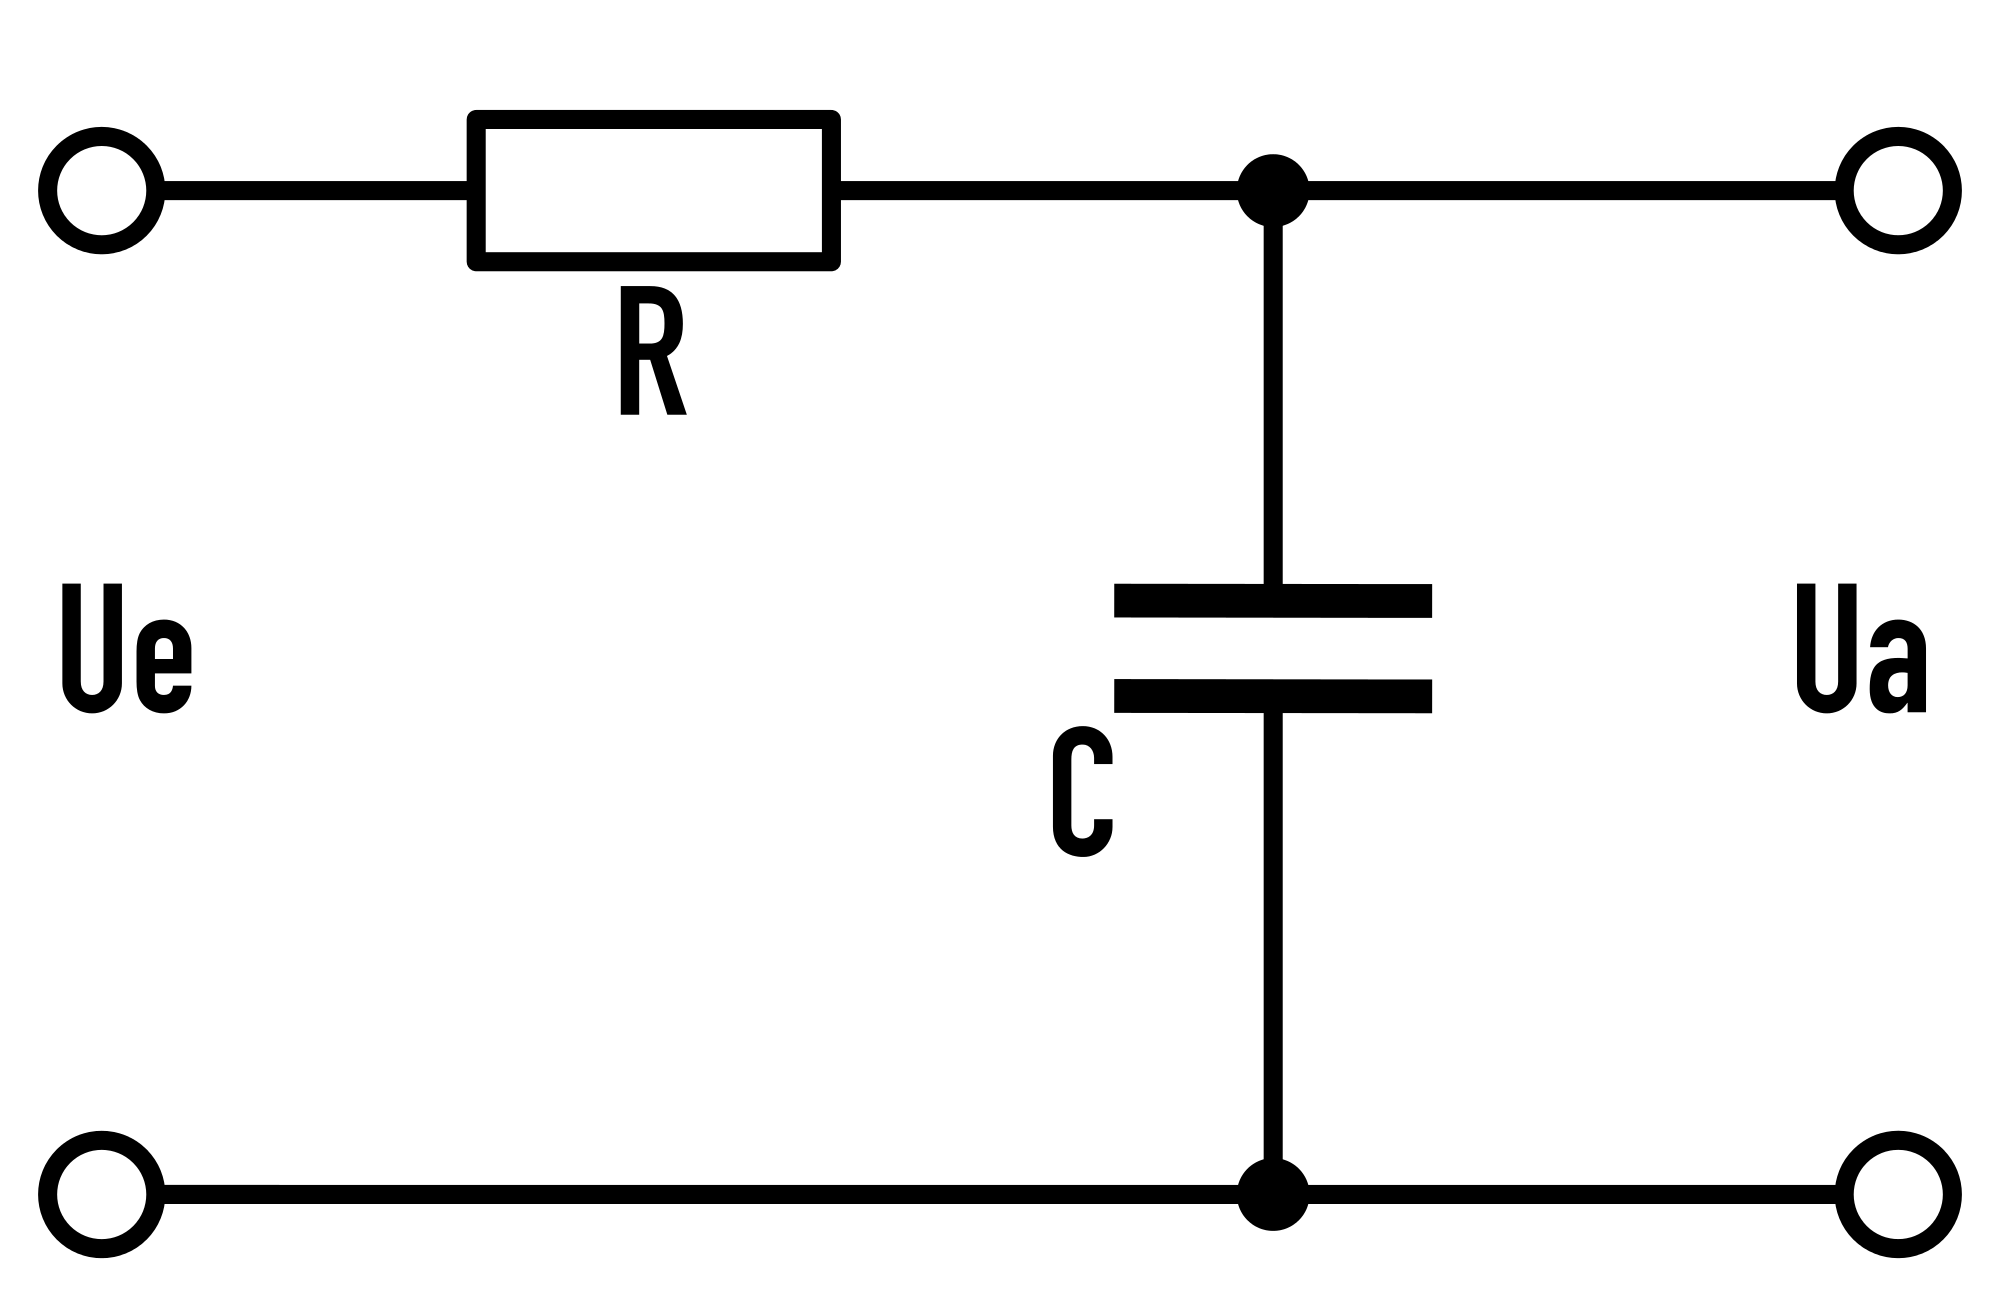
\includegraphics[scale=0.1]{Bilder/Vorversuch1/Tiefpass_Schaltbild.png}
\caption[test]{Schaltbild\footnotemark eines Tiefpasses.}
\label{fig:Tiefpass_Schaltbild}
\end{figure}
%\footnotetext{Quelle: \url{http://de.wikipedia.org/wiki/Tiefpass}}
\footnotetext{Quelle: http://de.wikipedia.org/wiki/Tiefpass}

Mit einem \SI{1,5}{k \Omega} Widerstand und einem \SI{100}{nF} Kondensator wird ein Tiefpass zusammengesetzt. Mit einem Frequenzgenerator wird eine sinusförmige Wechselspannung an den Tiefpass angelegt. Abbildung \ref{fig:Tiefpass_Schaltbild} zeigt das entsprechende Schaltbild. Die angelegte Frequenz wird von \SI{10}{Hz} bis \SI{10000}{Hz} durchgefahren und dabei werden die an den Tiefpass angelegte und die durch den Tiefpass gefilterte Wechselspannung auf dem Oszilloskop und an einem Multimeter gemessen.

\subsubsection{Untersuchung der Filter des Lockin-Verstärkers}
Das Referenzsignal des Lockin-Verstärkers wird auf einen Eingang des Lockin-Verstärkers gelegt. Die Filterfrequenz wird auf $f_0 = \SI{1000}{Hz}$ eingestellt. Es werden alle drei Filter (Tiefpass-, Hochpass- und Bandpassfilter) des Lockin-Verstärkers vermessen, indem jeweils die Frequenz des Referenzsignals durchgefahren und die integrierte Spannungsausgabe des Lockin-Verstärkers gemessen wird. Alle Einstellungen sind in Tabelle \ref{tab:vor2} aufgelistet

\begin{table}[H]
\centering
\begin{tabular}{|c|c|}
\hline 
Amplitude $U_0$ & \SI{0,1}{V} \\
\hline 
Verstärkung $s$ & \SI{200}{mV} \\ 
\hline 
Phasenschieber & $\varphi = 0$ \\ 
\hline 
Filterfrequenz $f_0$ & \SI{1000}{Hz} \\ 
\hline 
Güte Q & 1 \\ 
\hline
Integrationszeit $T_I$ & \SI{300}{ms} \\ 
\hline 
\end{tabular} 
\caption{Einstellungen zur Untersuchung der internen Filter}
\label{tab:vor2}
\end{table}

\subsubsection{Signalfiltern mit Tiefpass und Hochpass}
Mit einem Frequenzgenerator wird eine niedrige Frequenz erzeugt und an einen Eingang des Lockin-Verstärkers gelegt. An den anderen Eingang des Lockin-Verstärkers wird das Referenzsignal des Lockin-Verstärkers gelegt. Mit dem Oszilloskop werden sowohl das Signal des Frequenzgenerators, das Referenzsignal und die Überlagerung der beiden Signale, die der Lockin-Verstärker auf dem SIG.MON Ausgang ausgibt, betrachtet\\
Nun wird jeweils ein Oszilloskopbild im Modus "FLAT","Tiefpass" und "Hochpass" aufgenommen. Dafür wurden zuerst Frequenzen von \SI{100}{Hz} und \SI{8000}{Hz} verwendet. Zur besseren Darstellung auf dem Oszilloskop wurden danach nochmal 3 Bilder mit den Frequenzen \SI{200}{Hz} und \SI{4000}{Hz} aufgenommen. Beide Bilderreihen wurden ausgewertet.\\
Die Filterfrequenz stand weiterhin auf $f_0 = \SI{1000}{Hz}$. Die Eingangspannungen wurden so eingestellt, dass eine Spannung von 0.5V nicht überschritten wurde. Alle anderen Einstellungen wurden aus den voherigen Versuchen übernommen.

\subsubsection{Zeitkonstante und Empfindlichkeit}

Der Lockin-Verstärker integriert das Signal über einen einstellbaren Zeitraum, um so die Schwingung aufgrund der Orthogonalitätsbedingung aus dem Ausgangssignal zu integrieren. \\
Die Empfindlichkeit $s$ des Lockin-Verstärkers wird angegeben in der Spannung, die auf \SI{10}{V} verstärkt wird, sodass sich der Verstärkungsfaktor zu $v = \frac{\SI{10}{V}}{s}$ berechnet. \\
Das Referenzsignal wird auf den Eingang des Lockin-Verstärkers gelegt. Die Frequenz des Referenzsignals wird durchgefahren, um ein geeignetes Verhältnis zwischen Referenzfrequenz und Integrationszeit zu finden. Tabelle \ref{tab:Zeitkonst_Einstellungen} zeigt die verwendeten Einstellungen.

\begin{table}[H]
\centering
\begin{tabular}{|c|c|}
\hline 
Integrationszeit $T_I$ & \SI{10}{ms} \\ 
\hline 
Amplitude $U_0$ & \SI{0,5}{V} \\
\hline 
Verstärkung $s$ & \SI{200}{mV} \\ 
\hline 
Phasenschieber & $\varphi = \frac{\pi}{2}$ \\ 
\hline 
\end{tabular} 
\caption{Einstellungen zur Bestimmung einer geeigneten Zeitkonstanten und Empfindlichkeit.}
\label{tab:Zeitkonst_Einstellungen}
\end{table}

\subsection{Hauptversuch}

\subsubsection{Messung des Supraleiters}
Der Messstab mit dem Supraleiter wird zunächst mit einer Pumpe evakuiert und anschließend mit Helium als Kontaktgas befüllt. Das Ende des Stabes, an dem die Messeinrichtung sitzt, wird zum Kühlen in einen mit flüssigem Stickstoff gefüllten Dewar getaucht und auf ca. \SI{80}{K} gekühlt. Für die Messung wird anschließend der Messstab aus dem Stickstoff herausgezogen, allerdings nur so weit, dass die Erwärmungsrate $\frac{\Delta T}{\Delta t}$ unter \SI{0,1}{K/s} bleibt. Dies ist wichtig, um sicherzustellen, dass zu jedem Zeitpunkt eine möglichst homogene Temperaturverteilung gegeben ist. Während der Erwärmung von \SI{80}{K} auf ca. \SI{120}{K} wird die Temperatur und die Differenzspannung zwischen den beiden Empfängerspulen des Hartshorn-Spulensystems gemessen. \\
Diese Messung wird einmal ohne Probe als Untergrundmessung zur Korrektur und zweimal mit dem Supraleiter durchgeführt: Einmal mit einer Phasenverschiebung zwischen Eingangssignal und Referenzsignal des Lockin-Verstärkers von $\varphi = 0$ bzw. $\varphi = \pi$ und einmal mit einer Phasenverschiebung von $\varphi = \frac{\pi}{2}$, sodass der Realteil ($\varphi = 0$) und der Imaginärteil ($\varphi = \frac{\pi}{2}$) der Suszeptibilität gemessen werden.

\subsubsection{Phasenkalibration}
\begin{figure}[H]
\centering
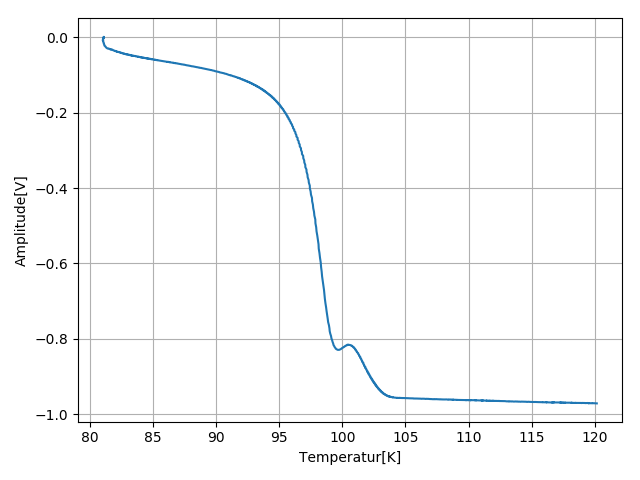
\includegraphics[scale=0.5]{Bilder/Haupt_Supra/Kalialt.png}
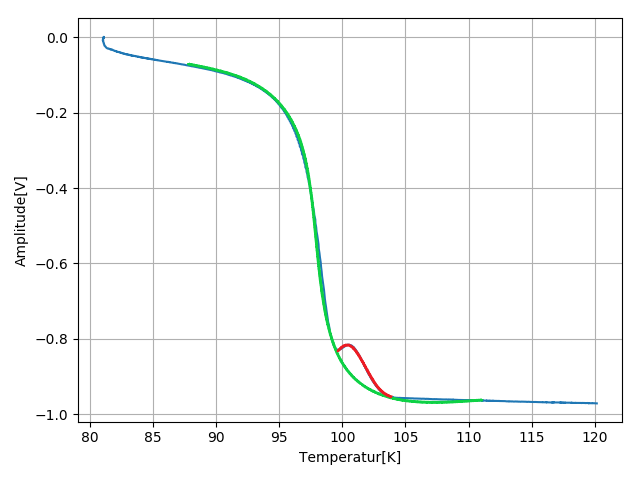
\includegraphics[scale=0.5]{Bilder/Haupt_Supra/Kalialt_2.png}
\caption{Ursprüngliche Phasenkalibration, bei der die Spannung mithilfe der Phase auf 0 kalibriert wurde. Im rechten Bild wurde der Verlauf von $\chi'$ in grün und der von $\chi''$ in rot qualitativ gekennzeichnet.}
\label{fig:Supra_Kalialt}
\end{figure}


Um Real- und Imaginärteil möglichst unabhängig voneinander betrachten zu können muss die Phase möglichst genau auf $90^\circ$ bzw. auf $0^\circ$ kalibriert werden. Ursprünglich sollte dies mithilfe der Tatsache geschehen, dass für den Supraleiter
\begin{equation}
\chi_C = -1-i\cdot 0
\end{equation}
gilt, der Imaginärteil also 0 ist.\\
Man verucht also auf $90^\circ$ so zu kalibrieren, dass der Offset \SI{0}{V} beträgt. Eine Messreihe mit einer solchen Kalibration ist in Abbildung \ref{fig:Supra_Kalialt} dargestellt.\\
Das Problem dabei ist, dass die Position des Dewar-Gefäßes das Magnetfeld der Spulen beeinflusst. Da diese Postition mehrfach während des Versuches geändert werden muss, entsteht ein Offset, der nicht durch das Potentiometer ausgeglichen wurde. Den Einfluss kann man zum Beispiel durch eine Änderung in der Spannung ganz am Anfang der Messung beobachten, wo das Spulensystem leicht aus dem Dewar angehoben wird, um den Erwärmungsvorgang zu starten.\\
Bei der 0-Kalibration kalibriert man somit nicht auf $90^\circ$, sondern auf irgendeinen anderen Wert. Dies zeigt sich in Abbildung \ref{fig:Supra_Kalialt} durch das gleichzeitige Auftreten der $\chi'$-Kurve (Änderung von $\chi' = -1$ zu $\chi' << 1$ an der kritischen Temperatur) und des $\chi''$-Peaks.\\
\\
Um die Phase besser kalibriern zu können wurde ein alternatives Vervahren verwendet. Es wurde zuerst für eine Phase von $90^\circ$ ein Kurvenverlauf aufgezeichnet und dann geschaut, wie sich dieser Verlauf ändert, wenn man die Phase leicht verringert. Dies wird solange wiederholt, bis der Unterschied vor und hinter der Sprungtemperatur, der durch die $\chi'$-Kurve entsteht, verschwindet. Dieses Verfahren ist in Abbildung \ref{fig:Supra_Kali} anhand von 4 Schritten dargestellt.\\
Damit ist der Aufbau auf den Imaginärteil kalibriert. Um den Realteil zu messen wird die Grobeinstellung der Phase von $0^\circ$ auf $90^\circ$ gestellt.

\begin{figure}
\centering
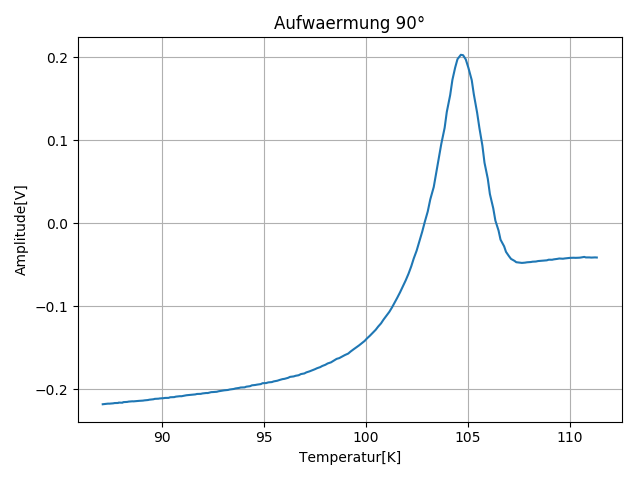
\includegraphics[scale=0.5]{Bilder/Haupt_Supra/Kal_2.png}
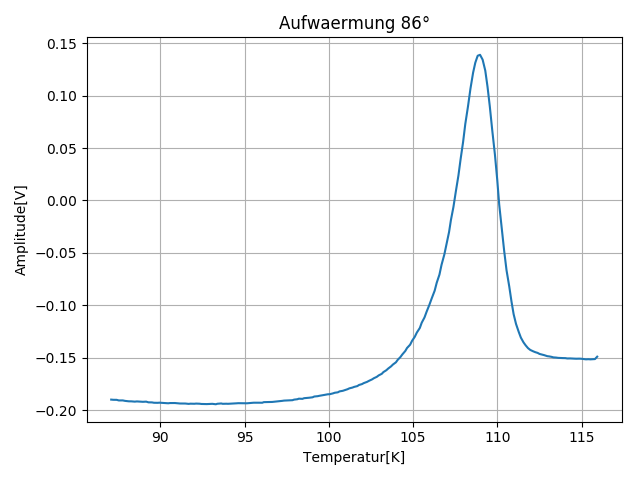
\includegraphics[scale=0.5]{Bilder/Haupt_Supra/Kal_0.png}
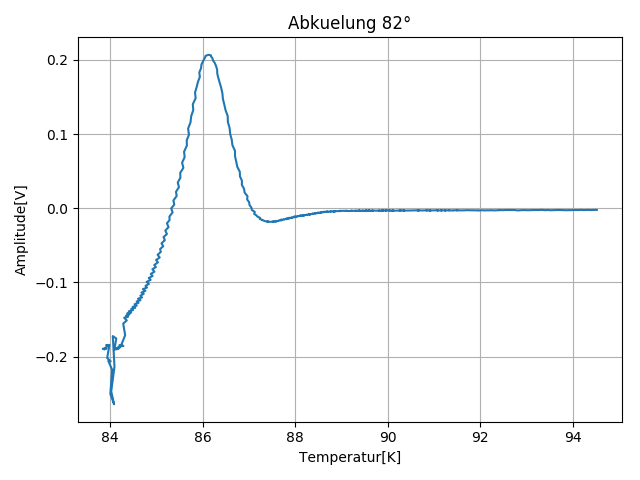
\includegraphics[scale=0.5]{Bilder/Haupt_Supra/Kal_1.png}
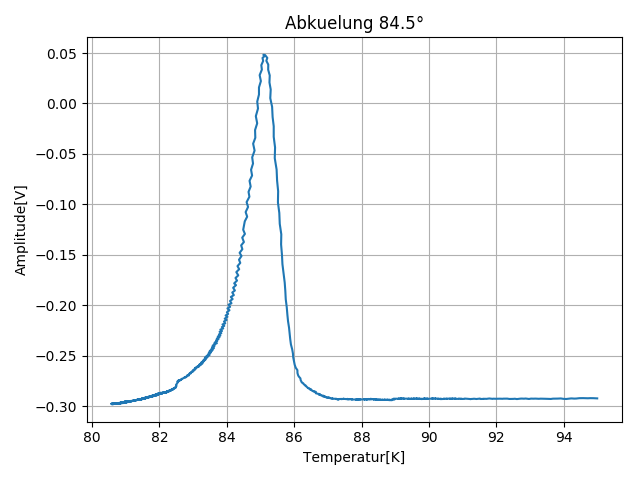
\includegraphics[scale=0.5]{Bilder/Haupt_Supra/Kal_3.png}
\caption{Alternative Phasenkalibration. \textbf{Oben links:} Aufwärmvorgang mit Phaseneinstellung von $90^\circ$. Der Verlauf der $\chi'$-Kurve ist sichtbar. \textbf{Oben rechts:} Aufwärmvorgang mit etwas besserer Phase von $86^\circ$. $\chi'$-Kurve ist schwächer ausgeprägt. \textbf{Unten links:} Abkühlvorgang mit zu kleiner Phase von $82^\circ$. $\chi'$-Kurve ist wieder stärker ausgeprägt. \textbf{Unten rechts:} Abkühlvorgang mit entgültiger  Phase von $84.5^\circ$. Die Spannung hat vor und hinter dem Peak den gleichen Wert.}
\label{fig:Supra_Kali}
\end{figure}

\subsubsection{Einstellungen}
\begin{table}
\centering
\begin{tabular}{|c|c|}
\hline 
Integrationszeit $T_I$ & \SI{100}{ms} \\ 
\hline 
Sensitivität $s$ & \SI{500}{\mu V} \\ 
\hline
Filter & Bandpass \\
\hline
Güte & 1 \\
\hline
Referenz-/Filterfrequenz & \SI{380}{Hz} \\
\hline 
Feineinstellung Phase & $\varphi$ = 84.5$^{\circ}$ \\ 
\hline 
Messintervall & \SI{200}{ms} \\ 
\hline 
\end{tabular} 
\caption{Einstellungen für die Messung des Supraleiters.}
\label{tab:Supra_Einstellungen}
\end{table}

Die Einstellungen für den Hauptversuch müssen folgende Gleichung erfüllen:
\begin{equation}
C \chi' V_{Probe} (1-n_{probe})< s
\label{eq:C}
\end{equation}
wobei $\chi' < 5$ und $n_{probe} = 0.27$ vorgegebene Parameter sind. Das Probenvolumen wurde auf $V_{Probe} = \SI{22,90 \pm 0,05}{mm^3}$ bestimmt. Die Kalibrationskonstante kann über
\begin{equation}
C = \dfrac{2\pi f_R \mu_0 I_0 N_{sek} N_{prim}}{l_{sek} l_{prim}}
\end{equation}
mit $I_0 = \SI{1}{mA}$,$N_{sek} = 700$,$N_{prim} = 2046$,$l_{sek} = \SI{20}{mm}$,$l_{prim} = \SI{50}{mm}$ bestimmt werden. Diese hängt von der Referenzfrequenz ab, man bekommt also eine Beziehung zwischen $f_R$ und s. Mit einer Frequenz von $\SI{380}{Hz}$ ergibt die linke Seite von Gleichung \ref{eq:C} einen Wert $359\cdot 10^{-6}$, welcher kleiner als die vorgeschriebene Größe von $s = 500\cdot 10^{-6} s$ ist. Diese Frequenz kann also verwendet werden. Mit dieser Frequenz benötigt man eine Integrationszeit von $T_I = 100ms$ (vgl. Kapitel \ref{kap.vor4}).\\
\textbf{Anmerkung:} Es stellte sich während des Versuches heraus, dass die hier abgeschätzte Kalibrationskonstante deutlich zu klein war. Dadurch ist Bedingung \ref{eq:C} in Wirklichkeit nicht erfüllt, wodurch es zu Problemen bei der Messung der Probe kam und die Sentsitivität verdoppelt werden musste.\\
Alle Messeinstellungen sind nochmal in Tabelle \ref{tab:Zeitkonst_Einstellungen} aufgelistet.

\subsubsection{Messung der Probe}
Bei der Vermessung der GdAg$_{1-x}$Zn$_x$-Probe wird nur der Realteil gemessen. Die Messung wurde ebenfalls bei ca. \SI{80}{K} gestartet, jedoch bis ca. \SI{190}{K} aufgenommen. Wegen der falschen Kalibrationskonstante bei der Schnellauswertung wurde hier die angelegte Spannung zu groß, sodass die Sensitivität auf \SI{1}{mV} erhöht werden musste. Alle anderen Einstellungen wurden beibehalten.

\section{Ergebnisse}
\subsection{Vorversuche}
\subsubsection{Untersuchung eines Tiefpasses}
Die Messung des Tiefpasses wurde sowohl mit dem Multimeter als auch mit dem Oszilloskop aufgenommen. Dabei wurde mit dem Oszilloskop bei jeder Einstellung der Frequenz ein Bild gemacht, sodass die Auswertung der Oszilloskopdaten auch durch eine Anpassung an Eingangs- und Ausgangssignal geschehen kann. 

\paragraph{Multimeter}
Mit dem Multimeter wird die Effektivspannung von Eingangs- und Ausgangssignal gemessen.Da die Multimeterwerte um \SI{0,001}{V} geschwankt haben, wurde als Fehler auf diese Messungen
\begin{equation*}
\sigma _U = \dfrac{\SI{0,001}{V}}{\sqrt{12}}
\end{equation*}
als Gleichverteilungsfehler angenommen. Damit werden der Quotient $\frac{U_a}{U_e}$ und der Fehler durch gaußsche Fehlerfortpflanzung bestimmt. Die zugehörige Frequenz ist die eingestellte Frequenz, auf die der Digitalisierungsfehler
\begin{equation*}
\sigma _f = \dfrac{\SI{1}{Hz}}{\sqrt{12}}
\end{equation*}
angenommen wird. An diese Daten wird eine Anpassung der Form 
\begin{equation}
\dfrac{U_a}{U_e} = \dfrac{1}{\sqrt{1 + \left( \frac{f}{f_G} \right)^2}}
\label{eq:TiefpassFunktion}
\end{equation}
durchgeführt. 

\begin{figure}
\centering
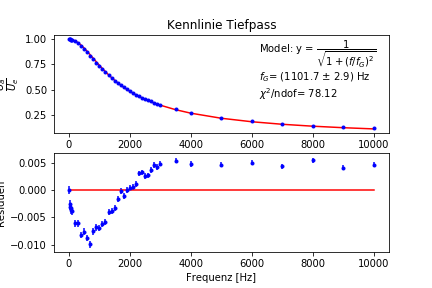
\includegraphics[scale=1]{Bilder/Vorversuch1/TiefpassMulti.png}
\caption[test]{Anpassung der Tiefpassfunktion an die mit dem Multimeter aufgenommenen Daten des selbstgebauten Tiefpasses.}
\label{fig:Tiefpass_Multi}
\end{figure}

Die Anpassung ist in Abbildung \ref{fig:Tiefpass_Multi} gezeigt. Der Verlauf der Daten zeigt, dass das Model durchaus richtig ist. Dennoch zeigen die Residuen gerade bei kleineren Frequenzen eine unbekannte Systematik.

\paragraph{Oszilloskop}
Die Oszilloskopdaten werden mittels Anpassung einer Cosinus-Funktion der Form
\begin{equation*}
U = U_0 \cdot \cos \left( 2 \pi \cdot f  + \varphi _0 \right)
\end{equation*}
ausgewertet. Für diese Anpassungen wird der Fehler auf die gemessene Spannung aus der Differenz der ersten beiden Spannungswerte geteilt durch $\sqrt{12}$ verwendet. Für den Fehler auf die Zeit wird der Abstand zweier Punkte geteilt durch $\sqrt{12}$ verwendet. Die Ergebnisse der Anpassungsparameter und die Fehler darauf sind nur sehr gering abhängig abhängig von den Fehlern, mit denen in diese Anpassung gegangen wird. Da nur die Ergebnisse dieser Parameter und deren Fehler weiter verwendet werden, reicht es, die Fehler für die Cosinus-Anpassung so grob abzuschätzen. \\
Mit den Ergebnissen für die Amplitude und die Frequenzen mit den Fehlern wird erneut eine Tiefpassfunktion (Gl. \ref{eq:TiefpassFunktion}) angepasst.

\begin{figure}
\centering
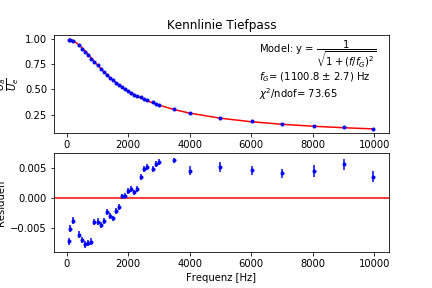
\includegraphics[scale=1]{Bilder/Vorversuch1/TiefpassOszi.png}
\caption[test]{Anpassung der Tiefpassfunktion an die mit dem Oszilloskop aufgenommenen Daten des selbstgebauten Tiefpasses.}
\label{fig:Tiefpass_Oszi}
\end{figure}

Die Anpassung ist in Abbildung \ref{fig:Tiefpass_Oszi} gezeigt. Der Verlauf der Daten zeigt, dass das Model durchaus richtig ist. Dennoch zeigen die Residuen gerade bei kleineren Frequenzen eine unbekannte Systematik. Die Ähnlichkeit zu der Anpassung an die Messung mit dem Multimeter (Abbildung \ref{fig:Tiefpass_Multi}) ist sehr auffällig.

\paragraph{Zusammenfassung}
Betrachtet man die Anpassungen an die mit dem Multimeter (Abbildung \ref{fig:Tiefpass_Multi}) und die mit dem Oszilloskop (Abbildung \ref{fig:Tiefpass_Oszi}) aufgenommenen Daten, fallen zwei Dinge auf:
\begin{enumerate}
\item Die beiden Anpassungen zeigen bei kleineren Frequenzen sehr ähnliche, starke Systematiken, die große $\chi ^2$/ndof bewirken
\item Die Grenzfrequenzen der beiden Anpassungen stimmen innerhalb ihrer Fehler überein
\end{enumerate}
Woher die Systematiken genau kommen ist nicht klar. Da diese aber in beiden Auswertungsmethoden zu sehen sind, ist davon auszugehen, dass sie dem Aufbau entstammen und nicht der Auswertungsmethode. \\
Dass die Grenzfrequenzen innerhalb ihrer Fehler übereinstimmen ermöglicht eine gewichtete Mittelung zu:
\begin{equation*}
f_G = \SI{1101,2 \pm 2,0}{Hz}
\end{equation*}
Die Bauteile des Tiefpasses sind vom Hersteller mit
\begin{equation*}
C = \SI{100 \pm 10}{nF}
\end{equation*}
\begin{equation*}
R = \SI{1500 \pm 15}{\Omega}
\end{equation*}
angegeben. Damit ergibt sich die Grenzfrequenz gemäß
\begin{equation*}
f_G^{Literatur} = \dfrac{1}{2 \pi RC}
\end{equation*}
und der Fehler gemäß
\begin{equation*}
\sigma _{f_G^{Literatur}} = f_G^{Literatur} \cdot \sqrt{\left( \dfrac{\sigma _R}{R} \right) ^2 + \left( \dfrac{\sigma _C}{C} \right) ^2}
\end{equation*}
zu:
\begin{equation*}
f_G^{Literatur} = \SI{1061 \pm 106}{Hz}
\end{equation*}
Der Fehler wird hauptsächlich durch den großen Fehler auf die Kapazität des Kondensators begründet. Damit stimmen Literaturwert und Messergebnis innerhalb ihrer Fehler überein.

\subsubsection{Untersuchung des Tiefpasses des Lockin-Verstärkers}

\begin{figure}
\centering
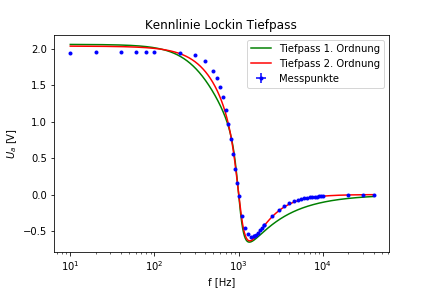
\includegraphics[scale=1]{Bilder/Vorversuch2/KennlinieTiefpass.png}
\caption[test]{Verlauf der Ausgangsspannung bei der Vermessung des Tiefpasses des Lockin-Verstärkers in Abhängigkeit von der Frequenz. In grün und rot sind die Anpassungen der Kennlinien von Tiefpässen 1. und 2. Ordnung.}
\label{fig:LockinTiefpass_Verlauf}
\end{figure}

Bei der Untersuchung der internen Filter wurde nur die Ausgangsspannung gemessen, nicht jedoch die Eingangsspannung. Diese wurde zwar konstant gehalten, um dies jedoch als mögliche Fehlerquelle auszuschließen, wird nur die Ausgangsspannung betrachtet[???-ka was damit gemeint ist]. \\
Den Verlauf der Ausgangsspannung in Abhängigkeit von der Frequenz zeigt Abbildung \ref{fig:LockinTiefpass_Verlauf}. Die Anpassungen der Kennlinien von Tiefpässen 1. bzw. 2. Ordnung sind mit $\chi ^2$/ndof von 2000 bzw. 500 und relativen Fehlern auf die Anpassungsparameter von bis zu $10^4$ nicht gelungen sind. Dennoch zeigen diese, wie in Abbildung \ref{fig:LockinTiefpass_Verlauf} gut erkennbar ist, dass es sich bei dem vermessenen internen Filter des Lockin-Verstärkers um einen Tiefpass 2. Ordnung handelt. \\
Wie bei einem Tiefpass erwartet, werden kleine Frequenzen durchgelassen und hohe Frequenzen unterdrückt. Dazwischen gibt es einen Übergangsbereich von ca. \SI{500}{Hz} bis ca. \SI{1500}{Hz}, in dem das Signal geschwächt durchgelassen wird bzw. teilweise auch mit $(-1)$ multipliziert wird.

\begin{figure}
\centering
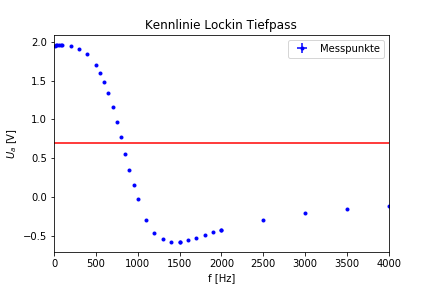
\includegraphics[scale=1]{Bilder/Vorversuch2/AblesenTiefpass.png}
\caption[test]{Verlauf der Ausgangsspannung bei der Vermessung des Tiefpasses des Lockin-Verstärkers in Abhängigkeit von der Frequenz in der Nähe der Grenzfrequenz. In rot ist die horizontale Linie eingezeichnet, bei deren Schnittpunkt mit den Daten die Grenzfrequenz liegt.}
\label{fig:LockinTiefpass_Ablesen}
\end{figure}

Da die Grenzfrequenz nicht aus den Anpassungen bestimmt werden kann, muss diese abgelesen werden. Dazu wird Abbildung \ref{fig:LockinTiefpass_Ablesen} betrachtet, in der die Frequenz zur Vereinfachung des Ablesens nicht logarithmiert und der Frequenzbereich eingeschränkt wurde. Die Grenzfrequenz wird dann abgelesen zu:
\begin{equation*}
f_G^{Tief} = \SI{830 \pm 14}{Hz}
\end{equation*}
Der Fehler wird dabei aus der Annahme einer Gleichverteilung zwischen den beiden Messpunkten um den Schnittpunkt abgeschätzt.

\subsubsection{Untersuchung des Hochpasses des Lockin-Verstärkers}

\begin{figure}
\centering
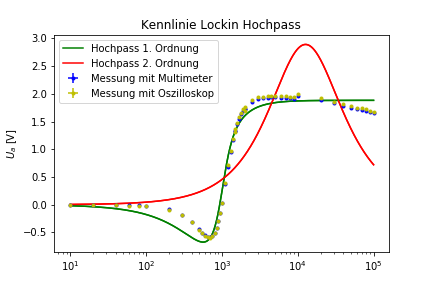
\includegraphics[scale=1]{Bilder/Vorversuch2/KennlinieHochpass.png}
\caption[test]{Verlauf der Ausgangsspannung bei der Vermessung des Hochpasses des Lockin-Verstärkers in Abhängigkeit von der Frequenz. In grün und rot sind die Anpassungen der Kennlinien von Hochpässen 1. und 2. Ordnung.}
\label{fig:LockinHochpass_Verlauf}
\end{figure}

Auch beim Hochpass wurde die Eingangsspannung nicht aufgenommen und deshalb nur die Ausgangsspannung betrachtet. \\
Auch hier sind die Anpassungen nicht gelungen. Dennoch zeigt Abbildung \ref{fig:LockinHochpass_Verlauf}, dass es sich bei dem vermessenen Hochpass des Lockin-Verstärkers um einen Hochpass 1. Ordnung handelt, da diese Anpassung die Daten deutlich besser beschreibt als die eines Hochpasses 2. Ordnung. \\
Wie bei einem Hochpass erwartet, werden kleine Frequenzen unterdrückt und hohe Frequenzen durchgelassen. Dazwischen gibt es wieder einen Übergangsbereich, wobei dieser bereits bei kleineren Frequenzen beginnt, nämlich bei ca. \SI{150}{Hz} und auch etwas weiter geht, bis ca. \SI{2}{kHz}. Abgesehen davon sieht der Übergangsbereich qualitativ dem Übergangsbereich des Tiefpasses ähnlich nur umgedreht.

\begin{figure}
\centering
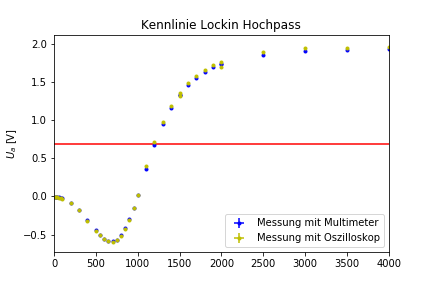
\includegraphics[scale=1]{Bilder/Vorversuch2/AblesenHochpass.png}
\caption[test]{Verlauf der Ausgangsspannung bei der Vermessung des Hochpasses des Lockin-Verstärkers in Abhängigkeit von der Frequenz in der Nähe der Grenzfrequenz. In rot ist die horizontale Linie eingezeichnet, bei deren Schnittpunkt mit den Daten die Grenzfrequenz liegt.}
\label{fig:LockinHochpass_Ablesen}
\end{figure}

Auch hier wird die Grenzfrequenz durch Ablesen bestimmt. Dazu ist in Abbildung \ref{fig:LockinHochpass_Ablesen} der Bereich um die Grenzfrequenz in nicht-logarithmischer Auftragung gezeigt. Die Grenzfrequenz wird dann abgelesen zu:
\begin{equation*}
f_G^{Hoch} = \SI{1200 \pm 29}{Hz}
\end{equation*}
Der Fehler wird dabei wieder aus der Annahme einer Gleichverteilung zwischen den beiden Messpunkten um den Schnittpunkt abgeschätzt.

\subsubsection{Untersuchung des Bandpasses des Lockin-Verstärkers}

\begin{figure}
\centering
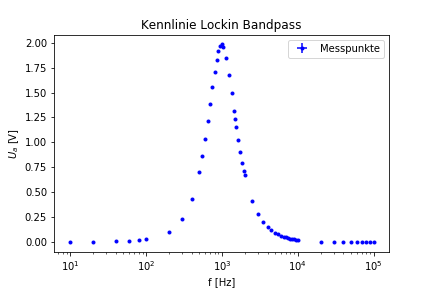
\includegraphics[scale=1]{Bilder/Vorversuch2/KennlinieBandpass.png}
\caption[test]{Verlauf der Ausgangsspannung bei der Vermessung des Bandpasses des Lockin-Verstärkers in Abhängigkeit von der Frequenz.}
\label{fig:LockinBandpass_Verlauf}
\end{figure}

Auch beim Bandpass wurde die Eingangsspannung nicht aufgenommen und deshalb nur die Ausgangsspannung betrachtet. \\
Hier wurden Anpassungen durchgeführt, da der Bandpass sehr wahrscheinlich durch Kombination der bereits vermessenen Tief- und Hochpass zusammengesetzt ist. \\
Abbildung \ref{fig:LockinBandpass_Verlauf} zeigt den gemessenen Verlauf der Ausgangsspannung in Abhängigkeit von der Frequenz. Wie bei einem Bandpass erwartet werden sowohl hohe als auch niedrige Frequenzen unterdrückt. In einem Bereich von ca. \SI{300}{Hz} bis ca. \SI{5}{kHz} werden die Frequenzen durchgelassen, wobei die Durchlassfunktion eine Gaußglockform hat.

\begin{figure}
\centering
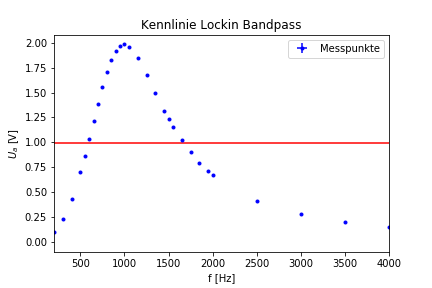
\includegraphics[scale=1]{Bilder/Vorversuch2/AblesenBandpass.png}
\caption[test]{Verlauf der Ausgangsspannung bei der Vermessung des Bandpasses des Lockin-Verstärkers in Abhängigkeit von der Frequenz in der Nähe der Grenzfrequenz. In rot ist die horizontale Linie eingezeichnet, bei deren Schnittpunkten die beiden den Peak begrenzenden Frequenzen liegen.}
\label{fig:LockinBandpass_Ablesen}
\end{figure}

Für die Bestimmung der Güte des Bandpasses werden die beiden den Peak begrenzenden Frequenzen $f_H$ und $f_L$ abgelesen. Mit diesen kann gemäß
\begin{equation*}
f_G = \sqrt{f_H \cdot f_L}
\end{equation*}
die Grenzfrequenz und mit
\begin{equation*}
Q = \dfrac{f_G}{f_H - f_L}
\end{equation*}
die Güte bestimmt werden. Die Fehler bestimmen sich nach gaußscher Fehlerfortpflanzung durch:
\begin{equation*}
\sigma _{f_G} = \sqrt{\left( \dfrac{\sigma _{f_H} \cdot f_H}{2 \cdot f_G} \right)^2 + \left( \dfrac{\sigma _{f_L} \cdot f_L}{2 \cdot f_G} \right)^2}
\end{equation*}
Die begrenzenden Frequenzen werden abgelesen zu:
\begin{equation*}
f_L = \SI{600 \pm 14}{Hz}
\end{equation*}
\begin{equation*}
f_H = \SI{1650 \pm 14}{Hz}
\end{equation*}
Der Fehler wird dabei wieder aus der Annahme einer Gleichverteilung zwischen den beiden Messpunkten um den Schnittpunkt abgeschätzt. \\
Damit bestimmen sich die Grenzfrequenz und die Güte zu:
\begin{equation*}
f_G = \SI{994 \pm 12}{Hz}
\end{equation*}
\begin{equation*}
Q = 0,948 \pm 0,021
\end{equation*}

\subsubsection{Zusammenfassung interne Filter des Lockin-Verstärkers}
Die Filter hatten alle qualitativ den erwarteten Verlauf in ihrer Übertragungsfunktion. Die Ergebnisse für die Grenzfrequenzen von Hoch- und Tiefpass liegen allerdings deutlich neben der eingestellten Frequenz von \SI{1000}{Hz}. Die Ursache davon ist unbekannt. \\
Dennoch stimmt die Grenzfrequenz des Bandpasses innerhalb ihres Fehlers mit der Erwartung von erneut \SI{1000}{Hz} überein. Der Messwert für die Güte liegt ca. 2,45$\sigma$ neben dem eingestellten Wert von 1. Da in den weiteren Messungen der Bandpass verwendet wurde, kann davon ausgegangen werden, dass der Lockin-Verstärker wie erwünscht funktioniert.

\subsubsection{Signalfiltern mit Tiefpass und Hochpass}
\begin{figure}
\centering
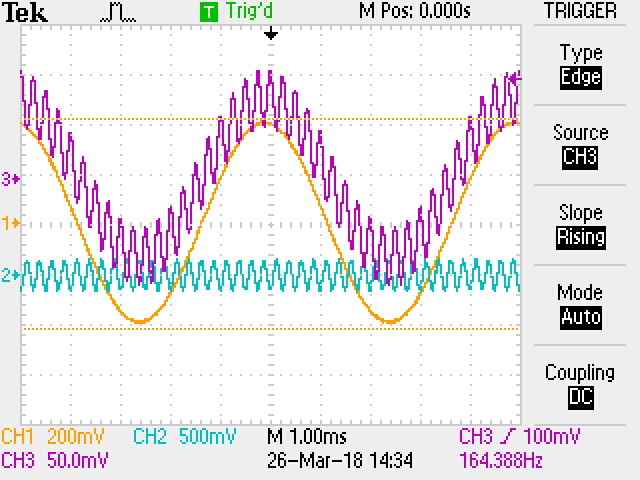
\includegraphics[scale=0.9]{Bilder/Vorversuch3/F0000TEK.JPG}
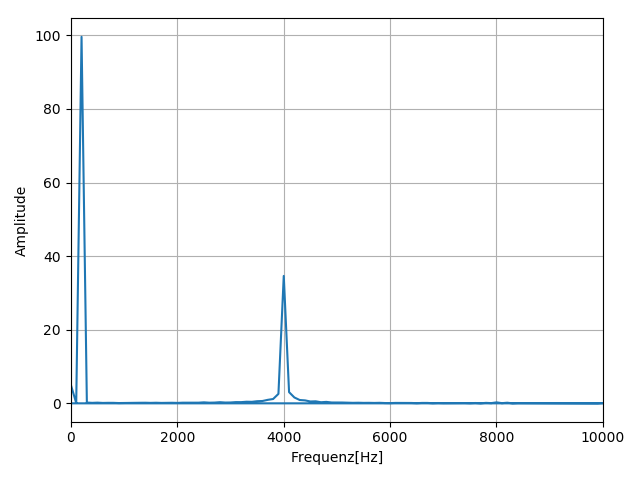
\includegraphics[scale=0.5]{Bilder/Vorversuch3/Vor3_0.png}
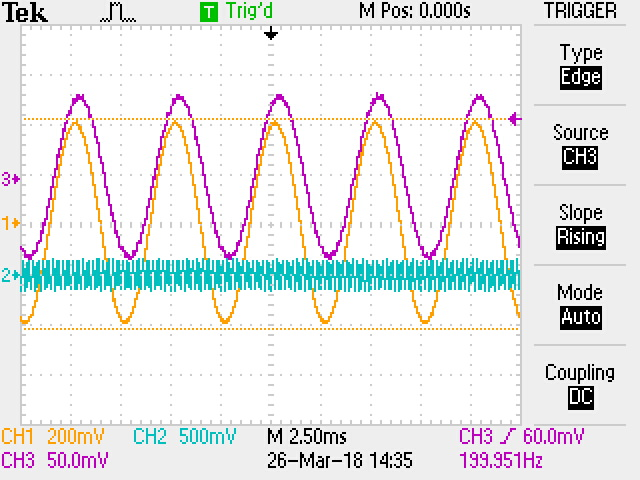
\includegraphics[scale=0.9]{Bilder/Vorversuch3/F0001TEK.JPG}
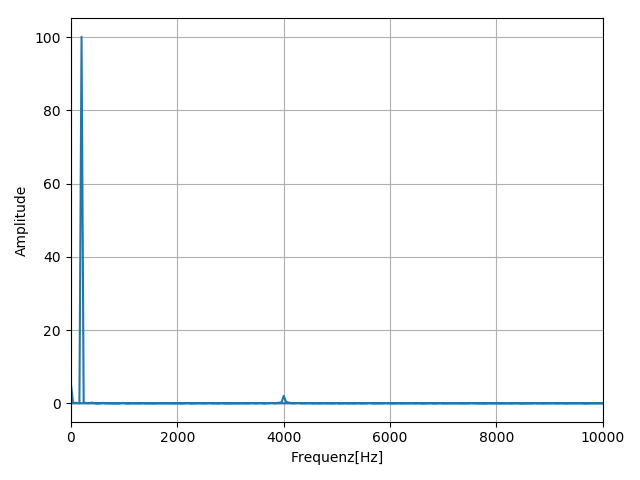
\includegraphics[scale=0.5]{Bilder/Vorversuch3/Vor3_1.png}
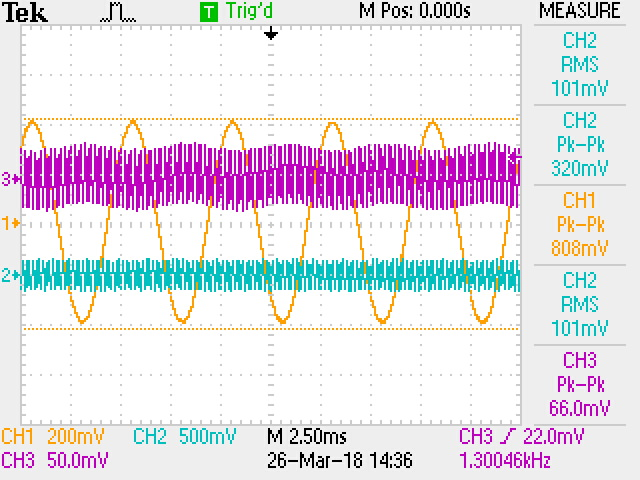
\includegraphics[scale=0.9]{Bilder/Vorversuch3/F0002TEK.JPG}
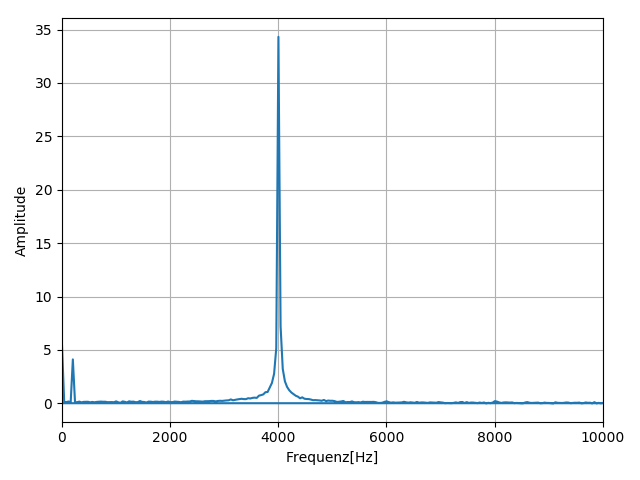
\includegraphics[scale=0.5]{Bilder/Vorversuch3/Vor3_2.png}
\caption{Osziloskopbilder zum Vorversuch zum Signalfiltern (Filterfrequenz: 1000Hz). \textbf{Oben:} Flat (kein Filter), \textbf{mitte:} Tiefpass, \textbf{unten:} Hochpass.
In allen Bildern ist an CH1 (orange) die kleine Frequenz (200Hz), CH2 (blau) die große Frequenz (4000Hz) und an CH3 die gefilterte Überlagerung der beiden Frequenzen angelegt.}
\label{fig:Vor3_Oszi}
\end{figure}

\begin{figure}
\centering
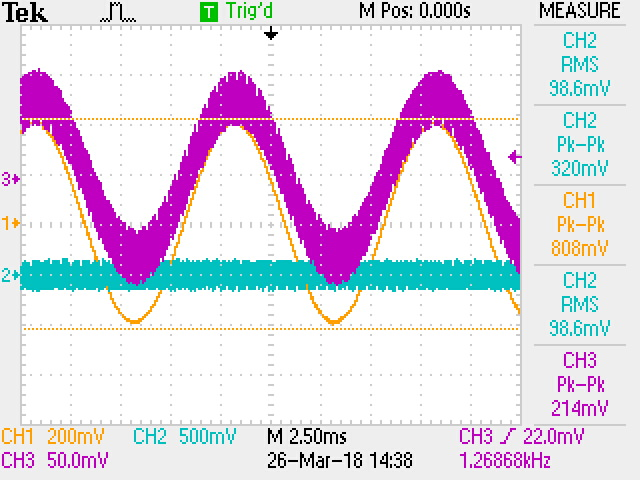
\includegraphics[scale=0.9]{Bilder/Vorversuch3/F0003TEK.JPG}
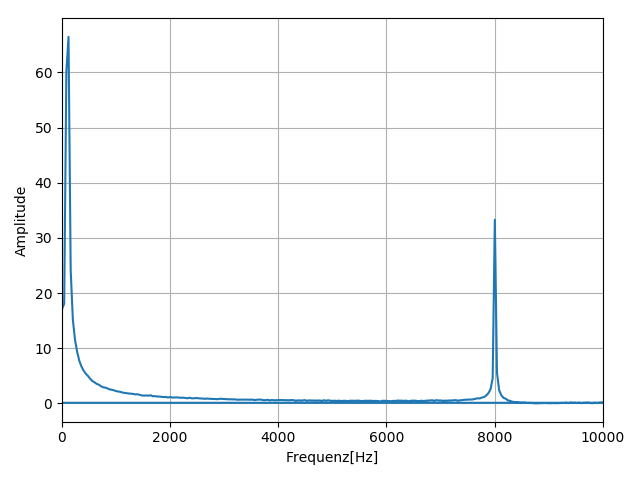
\includegraphics[scale=0.5]{Bilder/Vorversuch3/Vor3_3.png}
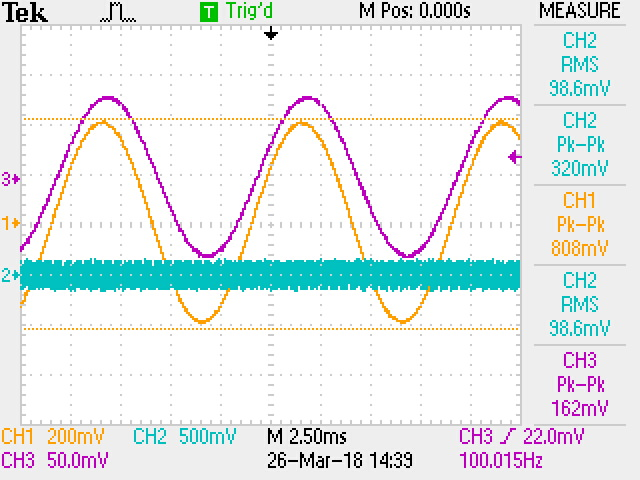
\includegraphics[scale=0.9]{Bilder/Vorversuch3/F0004TEK.JPG}
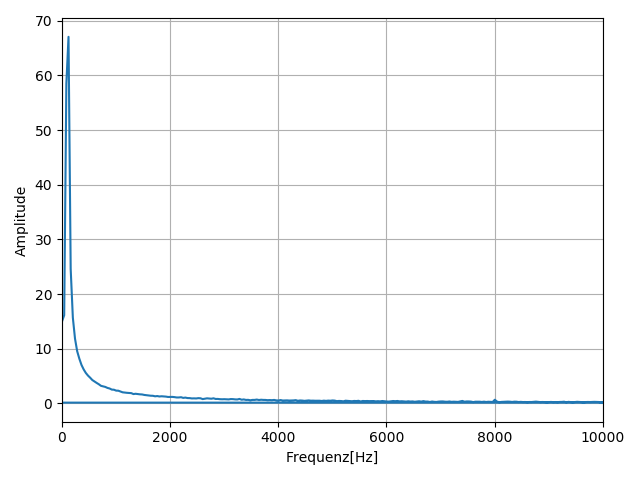
\includegraphics[scale=0.5]{Bilder/Vorversuch3/Vor3_4.png}
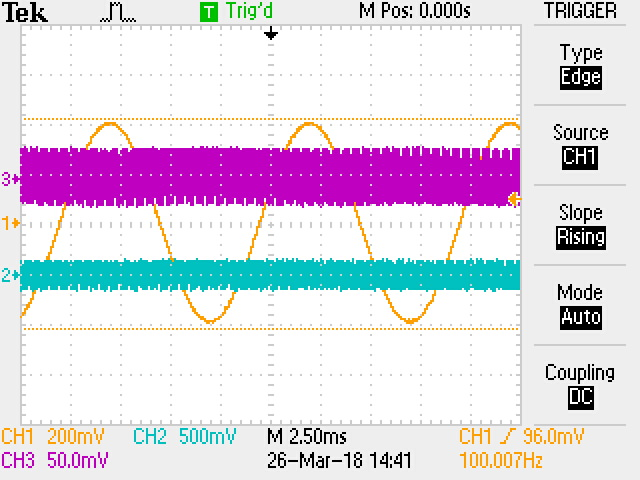
\includegraphics[scale=0.9]{Bilder/Vorversuch3/F0005TEK.JPG}
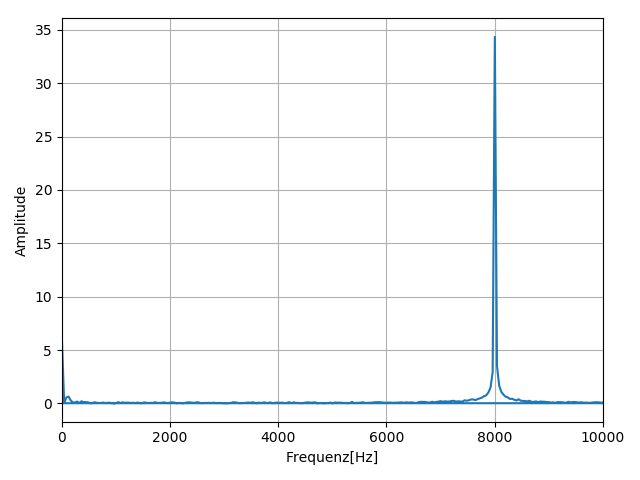
\includegraphics[scale=0.5]{Bilder/Vorversuch3/Vor3_5.png}
\caption{Osziloskopbilder zum Vorversuch zum Signalfiltern(Filterfrequenz: 1000Hz). \textbf{Oben:} Flat (kein Filter), \textbf{mitte:} Tiefpass, \textbf{unten:} Hochpass.
In allen Bildern ist an CH1 (orange) die kleine Frequenz (100Hz), CH2 (blau) die große Frequenz (8000Hz) und an CH3 die gefilterte Überlagerung der beiden Frequenzen angelegt.}
\label{fig:Vor3_Oszi2}
\end{figure}

\begin{table}
\centering
\begin{tabular}{|c|c|c|c|}
\hline
Filter & Frequenz & Höhe & rel. Höhe\\
\hline
kein & 100 & 66.4 & 1\\
\cline{2-4}
& 200 & 99.6 & 1\\
\cline{2-4}
& 4000 & 34.6 & 1\\
\cline{2-4}
& 8000 & 33.3 & 1\\
\hline
\hline
Tiefpass & 100 & 67.1 & $1.01\pm 0.01$\\
\cline{2-4}
& 200 & 100.1 & $1.01\pm 0.01$\\
\cline{2-4}
& 4000 & 2.1 & $0.06\pm 0.01$\\
\cline{2-4}
& 8000 & 0.7 & $0.02\pm 0.01$\\
\hline
\hline
Hochpass & 100 & 5.7 & $0.08\pm 0.01$\\
\cline{2-4}
& 200 & 4.1 & $0.04\pm 0.01$\\
\cline{2-4}
& 4000 & 34.3 & $0.99\pm 0.01$\\
\cline{2-4}
& 8000 & 34.3 & $1.03\pm 0.01$\\
\hline
\end{tabular} 
\caption{Ergebnisse der Peakhöhen der FFT-Spektren. Angegeben ist jeweils der verwendete Filter, die Frequenz, die absolute Peakhöhe (der genaue Wert hat keine Aussage) und die relative Peakhöhe verglichen mit den Höhen ohne Filter.}
\label{tab:Peakhohen}
\end{table}

In Abbildung \ref{fig:Vor3_Oszi} sind die Oszilloskopbilder für die Frequenzen 200Hz und 4000Hz zu sehen und in Abbildung \ref{fig:Vor3_Oszi2} die für die Frequenzen 100Hz und 8000Hz. Zur besseren Auswertung wurde jeweils eine Fast Fourier Transformation der dazugehörigen Daten durchgeführt. Diese ist jeweils neben dem Oszilloskopbild zu sehen. Aus den FFT-Spektren wurde die Peakhöhe abgelesen. Die Werte sind in Tabelle \ref{tab:Peakhohen} aufgelistet. Auf die Werte wurde ein Ablesefehler von 0.1 angenommen, welcher sich auf die rel. Höhe gaußisch fortpflanzt. 
\\
Bei den Aufnahmen ohne Filter (jeweils das oberste Bild) sieht man wie erwartet eine Überlagerung beider Frequenzen. Dabei ist die Intensität der niedrigen Frequenz deutlich höher. Dies liegt aber einfach daran, dass das Eingangsignal auf eine größere Amplitude eigestellt war.\\
\\
Bei den Aufnahmen mit dem Tiefpass ist die hohe Frequenz deutlich abgeschwächt und wird nurnoch mit einer relativen Höhe im einstelligen Prozentbereich registriert. Sie fällt zwischen der 4000Hz und 8000Hz Messung sogar nochmal um einen Faktor 3. Diese Abschwächung stimmt mit dem erwarteten Modell aus dem vorherigen Vorversuch überein. Die kleine Frequenz wird hier sogar ganz leicht verstärkt, dies spricht für das Ergebnis, dass die Güte leicht kleiner als 1 ist.
\\
Beim Hochpass ist dies wie erwartet genau anders herum. Hier werden die kleinen Frequenzen abgeschwächt. Die relative Höhe ist hier etwas ungenauer, da nur wenige Perioden in den Daten vorhanden sind. Deswegen ist hier auch der 100Hz Peak etwas stärker ausgeprägt als der 200Hz Peak.\\
Im Bild mit der 200Hz Frequenz (Abbildung \ref{fig:Vor3_Oszi} unteres Bild) kann man ausßerdem sehen, dass die kleine Frequenz um c.a $180^\circ$ phasenverschoben gegenüber der Eingangsfrequenz ist. Dies stimmt auch mit den Ergebnissen aus dem vorherigen Vorversuch überein. Leider ist die Auflösung der hohen Frequenz zu gering, sonst würde man dises Phänomen vermutlich auch beim Tiefpass bei der hohen Frequenz feststellen. 


\subsubsection{Zeitkonstante und Empfindlichkeit}
\label{kap.vor4}
Aus den Messeinstellungen ergibt sich ein in diesem Versuch verwendeter Verstärkungsfaktor von $v = 50$. Man erhält also die eigentlich gemessene Spannung, indem man die abgelesene verstärkte Spannung durch 50 teilt. In Abbildung \ref{fig:Vor4} sind die aufgenommenen Datenpunkte gegen die Frequenz aufgetragen. Die Spannungen haben immer um c.a 0.1V geschwankt, weswegen ein Ablesefehler von $0.1/50/\sqrt{12}$ auf die echten Spannungswerte angenommen wurde.\\
Zur besseren Auswertung wurde eine Anpassung an die Daten durchgeführt. Diese ist in Abbildung \ref{fig:Vor4_anpassung} zu sehen. Dabei stellt sich heraus, dass die Daten sehr gut einer $1/x^2$-Funktion folgen.\\
\\
Nun möchte man das optimale Verhältnis zwischen Integrationszeit $T_I$ und der Peraiodendauer T wissen, wobei gilt:
\begin{equation}
Ver = \dfrac{T_I}{T} = T_I \cdot f
\end{equation}
Während des Versuches wurde abgeschätzt, dass für die verwendete Integrationszeitvon $T_I = \SI{10}{ms}$ mindestens eine Frequenz von $f = \SI{1500}{Hz}$ benutzt werden muss, da sich die Werte ab dieser Frequenz kaum noch ändern. Dies führt zu einem schnell abgeschätzen Verhältnis von $Ver = 15$.\\
Beim Hauptversuch entstehen Spannungen im $\si{\mu V}$ Bereich (Empfindlichkeit auf $s = 500\mu V$ eingestellt). Der Einfluss auf die maximale Spannung durch die Integrationszeit sollte unter $1\%$ betragen, also einem Spannungsoffset von $5\mu V$. Es wird also visuell abgeschätzt, wann die Anpassung unter diesen Offset läuft(nach Abzug des Offsets (Anpassungsparameter d) der Anpassung, also wird nach einem y-Wert von $(0.0122\pm 0.0002)mV$ gesucht).  Dies ist der Fall bei $f = \SI{1610\pm 20}{Hz}$ (mit Ablesefehler). Daraus ergibt sich ein \textbf{minimales} Verhältnis von
\begin{equation*}
\boxed{T_I \cdot f = 16.1\pm 0.2}
\end{equation*}
Im Hauptversuch wurde eine Frequenz von \SI{380}{Hz} verwendet. Man benötigt also eine Integrationszeit von \SI{100}{ms}, da das Verhältnis sonst zu klein ist. Mit diesen Einstellungen ergibt sich ein Verhältnis von 
$38$. Die Bedingung ist also sehr gut erfüllt.
\begin{figure}
\centering
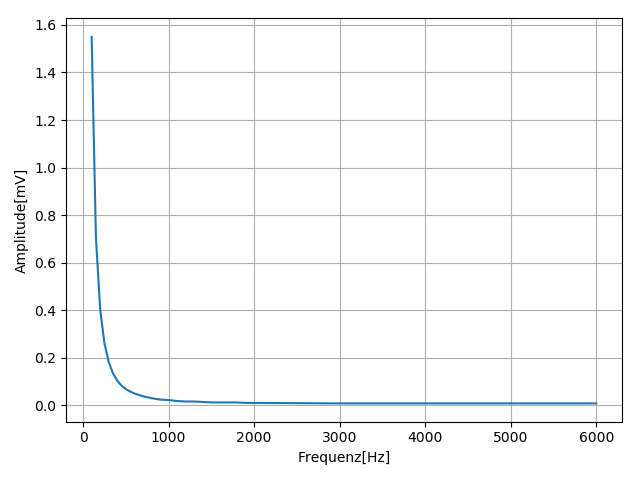
\includegraphics[scale=0.8]{Bilder/Vorversuch4/Vor4_0.png}
\caption{Aufgenommene Datenpunkte zur Betrachtung der Integrationszeit (T=10ms). Es wurde das echte Eingangsignal($U_{gemessen}/50$) gegen die Frequenz aufgetragen.}
\label{fig:Vor4}
\end{figure}

\begin{figure}
\centering
\includegraphics[scale=0.8]{Bilder/Vorversuch4/Vor4_1.png}
\includegraphics[scale=0.8]{Bilder/Vorversuch4/Vor4_2.png}
\caption{Anpassung an die Daten zur Zeitkonstante und eine Vergrößerung in den relevanten Bereich.}
\label{fig:Vor4_anpassung}
\end{figure}

\newpage
\subsection{Messung des Supraleiters}
Am Anfang von der $\chi'$-Messung wurden mehrere Messpunkte bei nahezu konstanter Temperatur aufgezeichnet. Aus diesen wird durch Mittelung und Bildung der Standardabweichung ein Fehler die Datenpunkte \textbf{aller} Messreihen bestimmt. Es ergab sich ein Fehler auf die Spannung von
\begin{equation*}
\sigma_U = 0.002V
\end{equation*}
und auf die Temperatur von
\begin{equation*}
\sigma_T = 0.01K
\end{equation*}
Diese Fehler wurden allgemein auf alle Datenpunkte angewendet.

\subsubsection{Untergrundmessung}
\begin{figure}
\centering
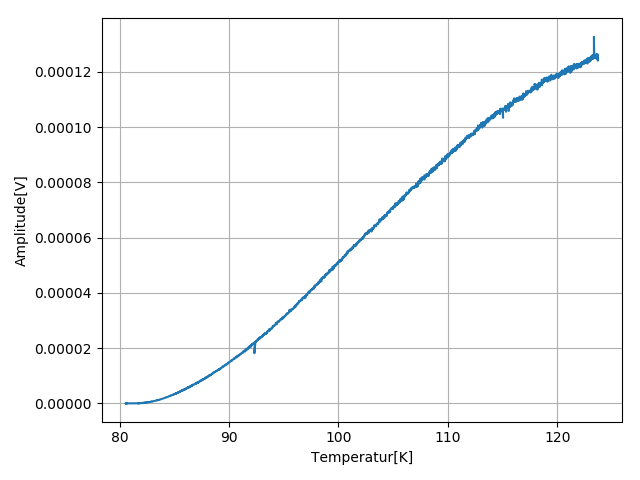
\includegraphics[scale=0.8]{Bilder/Haupt_Supra/Untergrund.png}
\caption{Untergrundmessung mit leerem Probenbehälter.}
\label{fig:Supra_Untergrund}
\end{figure}

In Abbildung \ref{fig:Supra_Untergrund} ist die Untergundmessung dargestellt. Am Anfang der Messung (bei nirdrigen Temperaturen) sieht man einen plötzlichen Anstieg der gemessenen Spannung. Dieser entsteht weider dadurch, dass der Stab leicht aus dem Dewar-Gefäß angehoben wird. Aus diesem Grund können nur Messwerte ab c.a 81.5K benutzt werden, falls ein Untergrundabzug durchgeführt wird.\\
Oberhalb dieser Temperatur folgen die Daten keinem einfachen Modell. Da die genaue Ursache dieses Verhaltens unbekannt ist, konnte keine Anpassung an die Daten durchgeführt werden. Stattdessen wird der Untergrund direkt von den Messreihen abgezogen.

\subsubsection{Auswertung der $\chi'$-Messung}
\begin{figure}
\centering
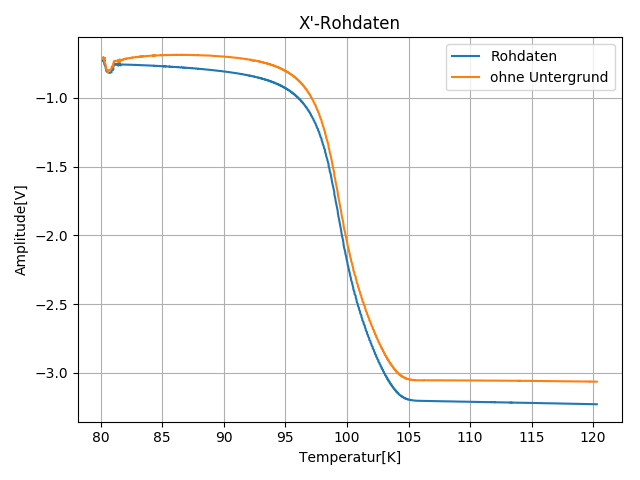
\includegraphics[scale=0.8]{Bilder/Haupt_Supra/X1roh.png}
\caption{Rohdaten der $\chi'$-Messung}
\label{fig:Supra_X1roh}
\end{figure}

\begin{figure}
\centering
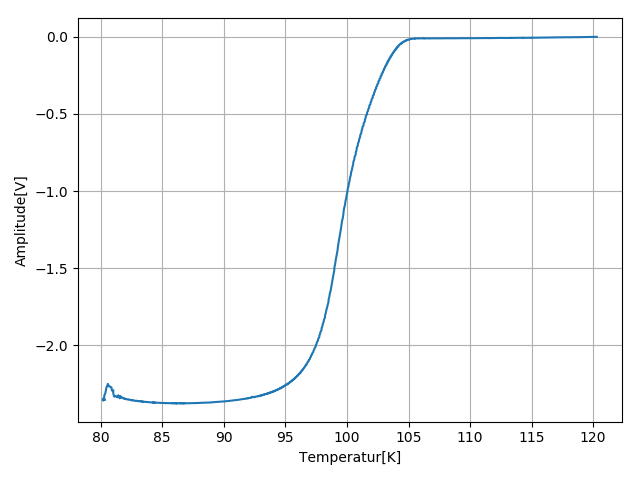
\includegraphics[scale=0.8]{Bilder/Haupt_Supra/X1_spiegel.png}
\caption{Vom Untergund korrigierte, gespiegelte und vom Offset bereinigte Daten der $\chi'$-Messung. Die y-Achse ist hier ansatzweise proportional zur Suszebtiblität.}
\label{fig:Supra_X1spiegel}
\end{figure}

\begin{figure}
\centering
\includegraphics[scale=0.5]{Bilder/Haupt_Supra/X1unten.png}
\includegraphics[scale=0.5]{Bilder/Haupt_Supra/X1oben.png}
\caption{Struktur in den Plateaus vor (linkes Bild) und hinter (rechtes Bild) der Sprungstelle in den Daten. Der Bereich zur Bestimmung der Plateauhöhe ist mit senkrechten Linien gekennzeichnet und liegt für den vorderen Berecih zwischen 82-87K und für den hinteren Bereich zwischen 107-120K.}
\label{fig:Supra_X1struct}
\end{figure}

Die Rohdaten der $\chi'$-Messung und die vom Untergrund bereinigten Daten sind in Abbildung \ref{fig:Supra_X1roh} dargestellt.\\
Da für diese Messung statt einer Phase von $0^\circ$ eine von $180^\circ$ verwendet wurde, sind die Daten an der X-Achse gespiegelt. Außerdem entsteht in dieser Messung ein relativ großer Offset.\\
Für $T>T_C$ ist der Supraleiter dia- oder paramagnetisch, es gilt also $|\chi'| << 1$. Falls man annimmt, dass für diese Temperaturen $|\chi'| \approx 0$ gilt, so kann man den Offset korrigieren. Da diese Korrektur für die Auswertung nicht relevant ist, wird sie nur durch abschätzen durchgeführt.
Die vom Untergund korrigierten, gespiegelten und vom Offset bereinigten Daten sind in Abbildung \ref{fig:Supra_X1spiegel} dargestellt. 

\paragraph{Bestimmung der Kalibrationskonstante}
Mit dem Wissen, dass $|\chi'| << 1$ für $T>T_C$ und $\chi' = 1$ für $T<T_C$ gilt, kann man die Kalibrationskonstante bestimmen. Dazu wird die Differenz der Spannungen vor und hinter dem Phasenwechsel gebildet.\\
Nach Abzug der Untergrundmessung bilden sich aber vor und hinter dem Phasenwechsel keine Plateaus aus. Stattdessen existiert immernoch eine Struktur in den Daten (vgl. Abbildung \ref{fig:Supra_X1struct}), welche die Bestimmung der jeweiligen Spannungen schwierig macht. Diese Sturktur kommt hauptsächlich dadurch, dass sich der Untergrund durch das Einbringen des Supraleiters leicht geändert hat.\\
Um trotzdem die Spannungsdifferenz ausrechnen zu können wird der Mittelwert dieser Plateaus gabildet. Die dafür ausgewählten Bereiche und die Position des Mittelwertes sind ebenfalls in Abbildung \ref{fig:Supra_X1struct} abgebildet.\\
\\
Der Bereich unter der Sprungtemperatur wurde so gewählt, dass die Streuung am Anfang vollständig rausgeschnitten wird und der Anstieg durch die Sprungstelle möglichst keinen Einfluss hat. Die Systematik durch die Sprungstelle beginnt ungefähr an der Stelle, an der die Spannung wieder anfängt zu steigen, anstatt abzufallen. Für den Bereich oberhalb der Sprungstelle wurde möglichst das ganze Plateau betrachtet, wobei eine kleine Bufferzone ausgelaasen wurde, um sicherzustellen, dass das Plateau wirklich erreicht wurde.\\
\\
Wegen der Struktur sind die Werte aber nicht gaußisch verteilt, und man kann den Fehler der Werte nicht durch Standardabweichung erhalten. Stattdessen wird eine Gleichverteilung zwischen dem Maximum und Minimum des ausgewählten Bereiches angenommen, da keine Aussage darüber getroffen werden kann, in welche Richtung die Daten durch den Untergrund verschoben werden. Die Spannungswerte sind in Tabelle \ref{tab:X1_const} aufgelistet.\\
Es gilt:
\begin{equation}
\Delta U = C \cdot v \cdot V_{Supra} \cdot \Delta\chi
\end{equation}
mit der Spannungsdifferenz U, der Kalibrationskonstante C, dem Verstärkungsfaktor $v=20000$ und des Volumens des Supraleiters $V_{Supra} =\SI{ 14.7\pm 0.3}{mm^3}$. Auf das Volumen wurde ein Gleichverteilungsfehler von $0.1/\sqrt{12}mm^3$ angenommen. Unter der Annnahme, dass $\Delta\chi \approx 1$ gilt, kann man daraus die Kalibrationskonstante berechnen:
\begin{equation}
C = \dfrac{\Delta U}{v\cdot V_{Supra}}
\end{equation}
Alle Fehler werden dabei gaußisch fortgepflanzt. Daraus erhält man das Endergebnis von
\begin{equation*}
C = \SI{8034.2\pm 34.7}{Vm^{-3}}
\end{equation*}

\begin{table}
\centering
\begin{tabular}{|c|c|}
\hline 
Messgröße & Wert \\ 
\hline 
Spannung unteres Plateau & \SI{-2.368\pm 0.009}{V} \\ 
\hline 
Spannung oberes Plateau & \SI{-0.006\pm 0.003}{V} \\ 
\hline 
Spannungsdifferenz & \SI{2.362\pm 0.009}{V} \\ 
\hline 
Kalibrationskonstante & \SI{8034.2\pm 34.7}{Vm^{-3}} \\ 
\hline 
\end{tabular} 
\caption{Spannungen an den beiden Plateaus und die daraus bestimmete Kalibrationskonstante}
\label{tab:X1_const}
\end{table}

\paragraph{Bestimmung der Sprungtemperatur}
Die Spungtemperatur befindet sich gerade an der Stelle, an der die Suszeptiblität am stäksten zunimmt. Deswegen wird jedem Messpunkt eine Steigung zugewiesen, indem eine lineare Anpassung an einen bestimmten Bereich um den Messpunkt herum angepasst wird. So kann man den Messpunkt bestimmen, an dem der Datenverlauf am steilsten ansteigt. In Tabelle \ref{tab:X1_anpassungen} sind die Ergebnisse der Anpassungen rund um die steilste Stelle aufgelistet. In Abbildung
\ref{fig:Supra_X1anpass} sind die Anpassungen zur steilsten Stelle und jeweils 2 Nachbarpunkten visualisiert.\\
Für den Anpassungsbereich wurden jeweils die nächsten 10 Nachbarpunkte in beide Richtungen gewählt, da sich die Stelle maximaler Steigung ab dieser Anpassungsgröße nicht mehr verändert. In Abbildung \ref{fig:Supra_X1anpassgross} ist die Auswrikung eines größeren Anpassungsbereiches mit 20 Nachbarpunkten gezeigt.\\
\\
Innerhalb der Fehler der Anpassungen liegen die beiden nächsten Nachabrpunkte im Bereich der maximalen Spannung. Deswegen wurden sie bei der Fehlerabschätzung berücksichtigt, indem gesagt wird, dass diese Werte den Fahler bestimmen. Dadurch ergibt sich ein Endergebnis von
\begin{equation*}
T_C = (99.38^{+0.04}_{-0.06}) K
\end{equation*}

\begin{table}
\centering
\begin{tabular}{|c|c|c|c|c|}
\hline
& $ 99.24 \pm 0.01 $ & $ 0.486 \pm 0.004 $ & $ -49.646 \pm 0.365 $ & $ 9.6 $\\
\hline
& $ 99.27 \pm 0.01 $ & $ 0.486 \pm 0.004 $ & $ -49.629 \pm 0.366 $ & $ 9.67 $\\
\hline
& $ 99.32 \pm 0.01 $ & $ 0.491 \pm 0.004 $ & $ -50.055 \pm 0.357 $ & $ 8.93 $\\
\hline
\hline
& $ 99.38 \pm 0.01 $ & $ 0.493 \pm 0.004 $ & $ -50.264 \pm 0.366 $ & $ 9.2 $\\
\hline
\hline
& $ 99.42 \pm 0.01 $ & $ 0.489 \pm 0.004 $ & $ -49.954 \pm 0.4 $ & $ 11.19 $\\
\hline
& $ 99.47 \pm 0.01 $ & $ 0.486 \pm 0.004 $ & $ -49.632 \pm 0.368 $ & $ 9.6 $\\
\hline
& $ 99.51 \pm 0.01 $ & $ 0.485 \pm 0.004 $ & $ -49.526 \pm 0.398 $ & $ 11.21 $\\
\hline
\end{tabular} 
\caption{Ergebnisse }
\label{tab:X1_anpassungen}
\end{table}

\begin{figure}
\centering
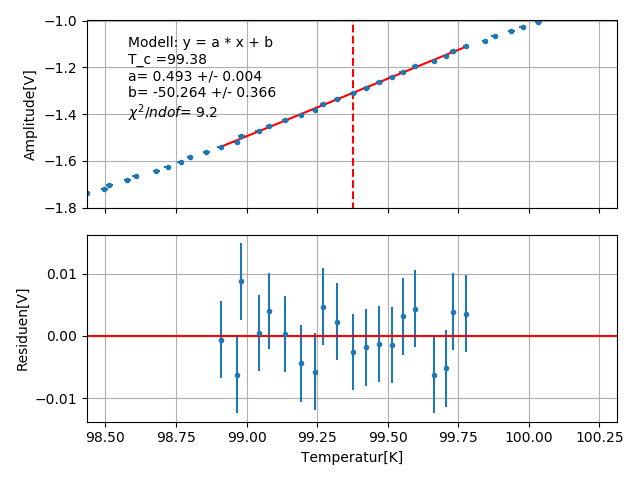
\includegraphics[scale=0.8]{Bilder/Haupt_Supra/X1_Steigung.png}
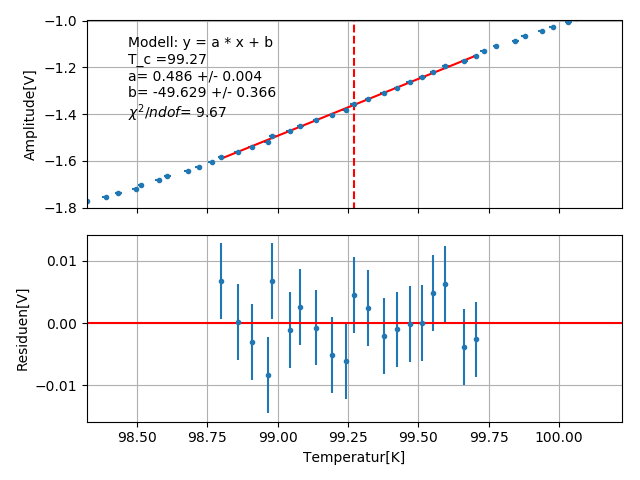
\includegraphics[scale=0.5]{Bilder/Haupt_Supra/X1_Steigung2.png}
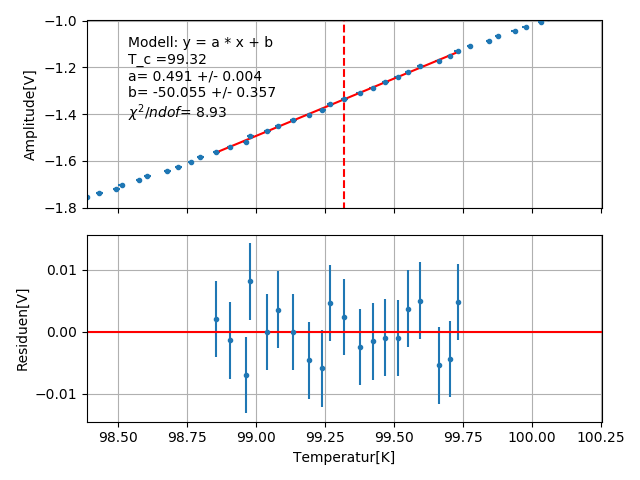
\includegraphics[scale=0.5]{Bilder/Haupt_Supra/X1_Steigung3.png}
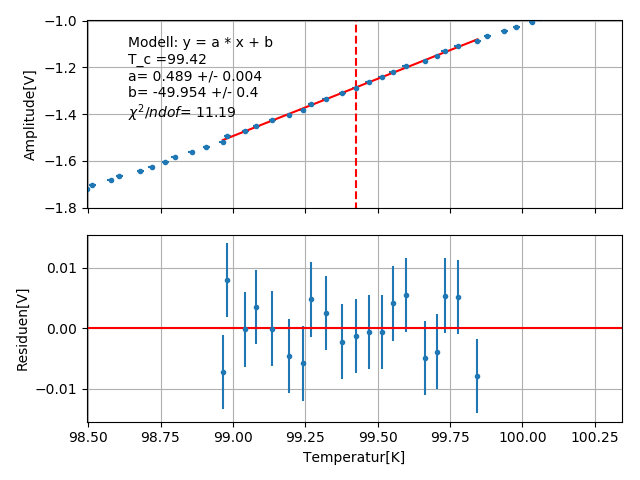
\includegraphics[scale=0.5]{Bilder/Haupt_Supra/X1_Steigung4.png}
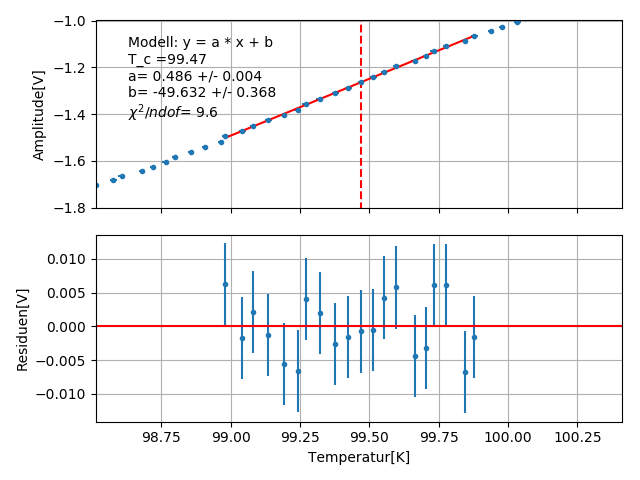
\includegraphics[scale=0.5]{Bilder/Haupt_Supra/X1_Steigung5.png}

\caption{Anpassungen an den Datenpunkt, die die größte Steigung ergeben hat (oben) und Anpassungen an die benachbarten Datenpunkte. Die zur Anpassung gehörigen Temperaturen $T_C$ wueden mit einer senkrechten Linie markiert.}
\label{fig:Supra_X1anpass}
\end{figure}

\begin{figure}
\centering
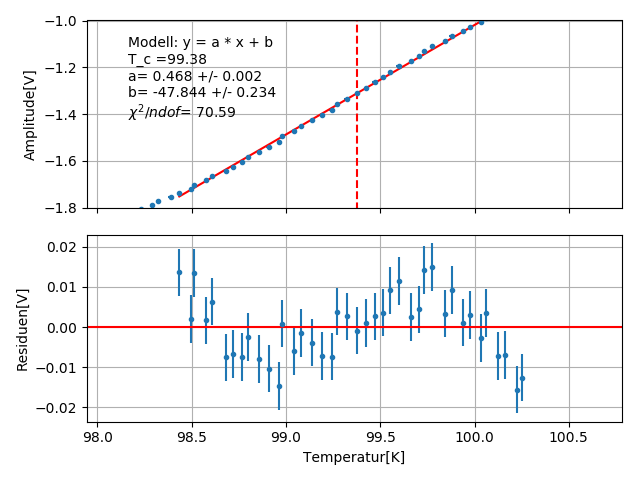
\includegraphics[scale=0.8]{Bilder/Haupt_Supra/X1_Steigung20.png}
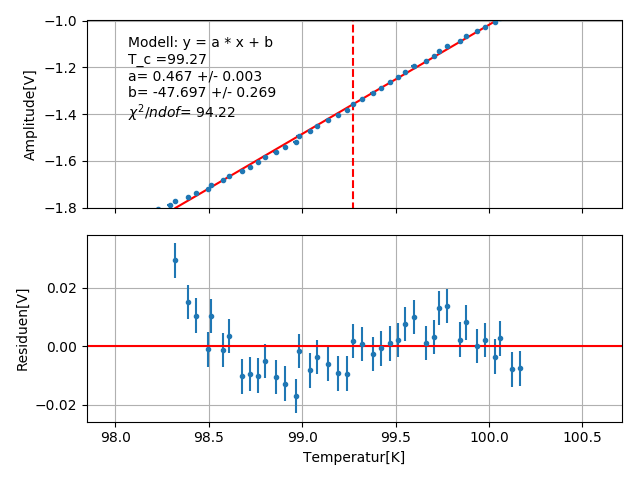
\includegraphics[scale=0.5]{Bilder/Haupt_Supra/X1_Steigung21.png}
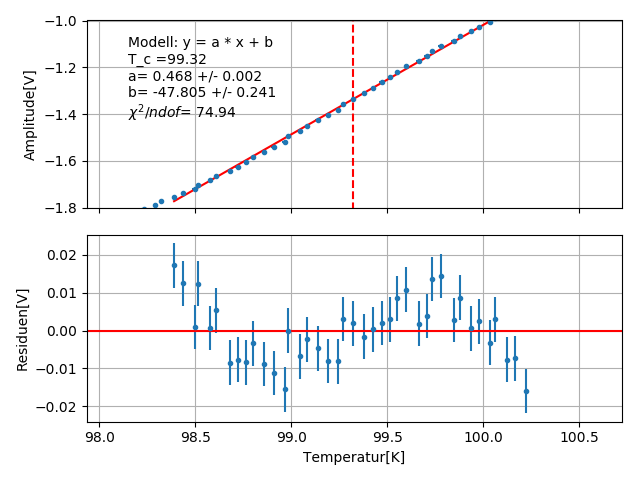
\includegraphics[scale=0.5]{Bilder/Haupt_Supra/X1_Steigung22.png}

\caption{Visualisierung der Folgen eines größeren Anpassungsbereiches (20 Nachbarpunkte) (oben: Maximalstelle, unten: nächste Nachbarn der Maximalstelle). Es ergibt sich die selbe Maximalstelle, allerdings ist in den Residuen eine Systematik zu erkennen, weswegen ein größerer Anpassungsbereich keinen wirklichen Sinn macht.}
\label{fig:Supra_X1anpassgross}
\end{figure}

\paragraph{Temperaturgradient}
\begin{figure}
\centering
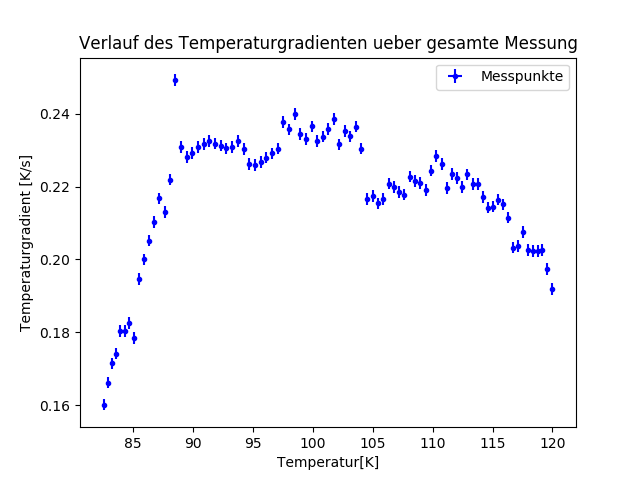
\includegraphics[scale=0.8]{Bilder/Haupt_Supra/X1_temp.png}
\caption{Temperaturgradient der $\chi'$-Messung.}
\label{fig:Supra_X1_temp}
\end{figure}

In Abbildung \ref{fig:Supra_X1_temp} ist der Temperaturgradient der Messung in Abhängigkeit von der Temperatur dargestellt. Im relevanten Bereich zwischen 98-100K erhält man durch eine Mittelung (Fehler aus Fehler auf den Mittelwert) eine ungefähre Abschätzung des Temperaturgradienten, der für die Abschätzung der Sprungtemperatur eine Rolle spielt:
\begin{equation*}
\dfrac{dT}{dt} = \SI{0.236\pm 0.005}{K/s}
\end{equation*}

\newpage
\subsubsection{Auswertung der $\chi''$-Messung}
\begin{figure}[h]
\centering
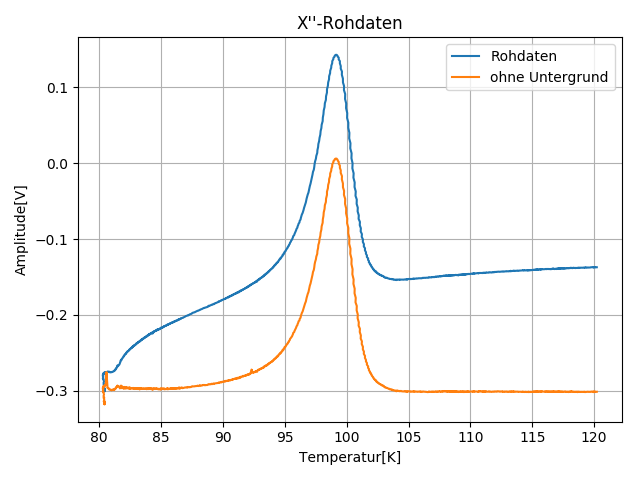
\includegraphics[scale=0.8]{Bilder/Haupt_Supra/X2roh.png}
\caption{Rohdaten und vom Untergrund bereinigte Daten der $\chi''$-Messung.}
\label{fig:Supra_X2roh}
\end{figure}

Die $\chi''$-Messung wurde ebenfalls vom Untergrund bereinigt. Dies ist zusammen mit den Rohdaten in Abbildung \ref{fig:Supra_X2roh} dargestellt.\\
\\
\paragraph{Kuvenverlauf}
Der Verlauf der $\chi''$-Messung kann folgendermaßen erklärt werden:\\
Da der Supraleiter leitend ist wird ein Strom in der Probe induziert. Durch die Änderung der Suszeptibilität ändert sich auch die Induktivität und somit die Spannung, die wieder in der Spule induziert wird. Diese Spannung ist um $90^\circ$ phasenverschoben und kann deswegen im Imaginärteil betrachtet werden. Je stärker die Änderung der Suszeptiblität ist, desto größer ist diese Spannung. Es entsteht ein Peak um die Sprungstelle.
\paragraph{Sprungtemperatur}
Die Sprungtemperatur stimmt hier mit der Peakposition überein. Um diese Postition zu bestimmen wird eine quadratische Funktion an die Spitze des Peaks angepasst. Der Fehler bestimmt sich durch Variation des Anpassungsbereiches, da durch die Unterschiedliche Flankensteigung des Peaks eine Systematik das Ergebnis ungenauer macht und deswegen der Fehler aus den Anpassungen auf die Position unter Umständen zu klein ist.\\
In Abbildung \ref{fig:Supra_X2anpassung} sind Anpassungen mit 3 verschiedenen Bereichen um die Peakspitze herum gezeigt. Die Ergebnisse dieser Anpassungen werden gemittelt. Den Fehler erhält man durch die maximale Abweichung einer Anpassung vom Mittelwert. Daraus ergibt sich das Endergebnis von
\begin{equation*}
T_C = \SI{99.12\pm 0.02}{K}
\end{equation*}

\paragraph{Temperaturgradient}
Mit der gleichen Methode wie bei der $\chi'$-Messung kann man hier den Temperaturgradienten bestimmen. Dies ist in Abbildung \ref{fig:Supra_X2temp} dargestellt. Es ergibt sich durch Mittelung der Werte zwischen 98K und 100K wieder ein relevanter Wert von 
\begin{equation*}
\dfrac{dT}{dt} = \SI{0.213\pm 0.004}{K/s}
\end{equation*}

\begin{figure}
\centering
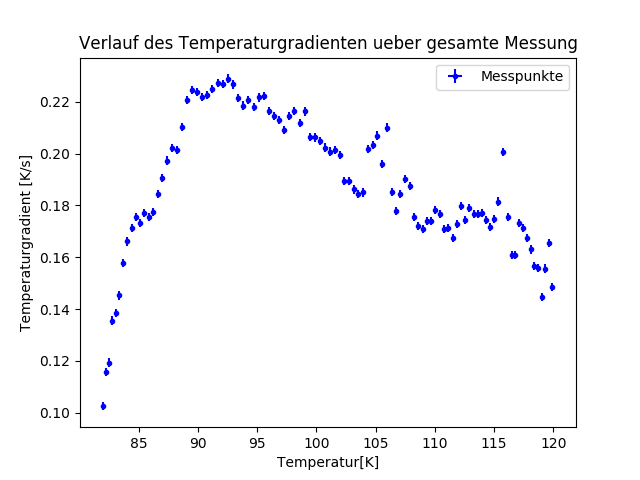
\includegraphics[scale=0.8]{Bilder/Haupt_Supra/X2_temp.png}
\caption{Temperaturgradient der $\chi''$-Messung.}
\label{fig:Supra_X2temp}
\end{figure}

\begin{figure}
\centering
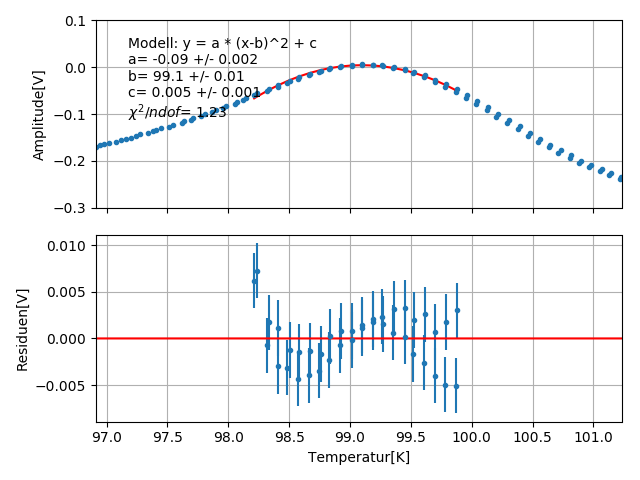
\includegraphics[scale=0.6]{Bilder/Haupt_Supra/X2_anpassung1.png}
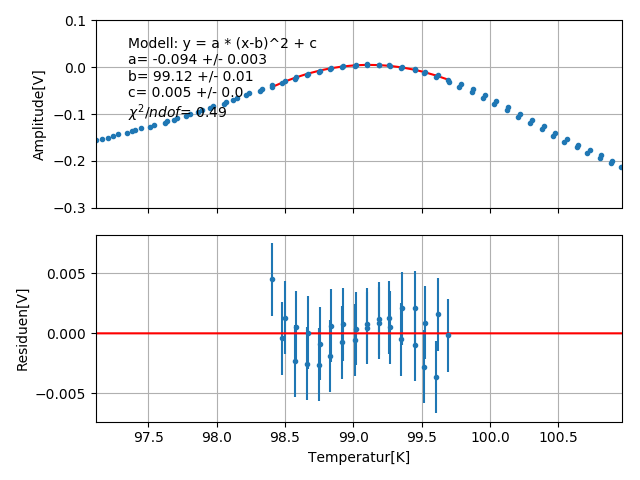
\includegraphics[scale=0.6]{Bilder/Haupt_Supra/X2_anpassung2.png}
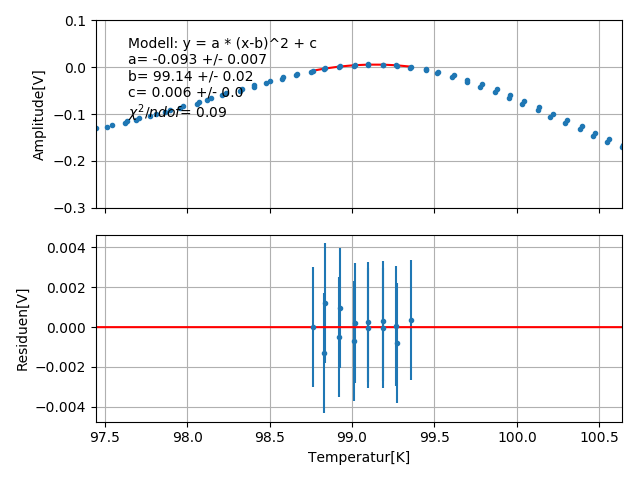
\includegraphics[scale=0.6]{Bilder/Haupt_Supra/X2_anpassung3.png}

\caption{Anpassungen an die Peakspitze mit 3 unterschiedlichen Anpassungsbereichen (14 Punkte, 28 Punkte und 40 Punkte).}
\label{fig:Supra_X2anpassung}
\end{figure}

\newpage
\subsubsection{Zusammenfassung der Messergebnisse}
Mithilfe der in der Versuchsanleitung gegebenen Daten für die Parameter des Aufbautes kann man den erwarteten Verstärkungsfaktor berechnen:
\begin{equation}
C = \dfrac{2\pi f_R \mu_0 I_0 N_{sek} N_{prim}}{l_{sek} l_{prim}}
\end{equation}
mit $f_R = \SI{380}{Hz}$,$I_0 = \SI{1}{mA}$,$N_{sek} = 700$,$N_{prim} = 2046$,$l_{sek} = \SI{20}{mm}$,$l_{prim} = \SI{50}{mm}$. Das Ergebnis ist in Tabelle \ref{tab:supra_ergebnis} zu finden.\\
Das Messergebnis weicht sehr stark vom Erwartungswert ab. Dies kann mehrere Gründe haben:
\begin{enumerate}
\item Fehler in der Methode zur Messwertbestimmung:\\
Es kann zum Beispiel sein, dass die Plateaus nicht den zugeordneten Suszeptiblitäten entspechen, sondern z.B die Suszebtiblität im supraleitenden Zustand $<1$ ist.
Dies ist zwar grundsätzlich möglich, es gibt aber eine Beobachtung, welche die Größenordnung des Messergebnisses bestätigt und eher den Erwartungswert hinterfragt:\\
Mithilfe von 
\begin{equation}
U_{max}^{lit} = C_{lit} \cdot \chi_{max} \cdot v \cdot (1-n_m) \cdot V_{Probe}
\end{equation}
und den verwendeten Werten für die SChnellauswertung während des Versuches von $\chi_{max} = 5$, $v = 20000$, $n_m = 0.27$ und $V_{Probe} = 22.9mm^3$ ergibt sich eine maximale Spannung von $U_{max} = 7.18V$. Mit dem sich aus der Messung ergebenen Wert für die Kalibrationskonstante ergibt sich hingegen eine Spannung von $U_{max} = 13.48V$. Bei der Messung mit diesen Einstellungen wurden Spannungen von über 10V erreicht, weswegen der Verstärkungsfaktor angepasst werden musste. Dies spricht eher für den berechneten Wert und gegen den Literaturwert.
\item Veraltete oder falsche Daten zur Berechnung des Erwartungswertes:\\
Da die Versuchanleitung schon etwas älter ist, kann auch nicht ausgeschlossen werden, dass die angegebenen Werte für veraltete Bauteile oder Proben gelten, wodurch sich ein anderer Kalibrationsfaktor ergibt. Dies ist wegen der oben ganannten Beobachtung wesentlich wahrscheinlicher.
\end{enumerate}

\begin{table}
\centering
\begin{tabular}{|c|c|c|}
\hline 
Messwert & Messergebnis & Erwartungswert \\
\hline 
Kalibrationskonstante C & $8034.2\pm 34.7$ & $4297$ \\ 
\hline 
Sprungtemperatur $\chi'$ & \SI{99.12\pm 0.02}{K} & \SI{92}{K} \\ 
\hline 
Sprungtemperatur $\chi''$ & $(99.38^{+0.04}_{-0.06}) K$ & \SI{92}{K} \\ 
\hline 
\end{tabular} 
\caption{Zusammenfassung der Messergebnisse zum Supraleiter und die dazu gehörigen Erwartungswerte.}
\label{tab:supra_ergebnis}
\end{table}

\paragraph{Sprungtemperatur}
Der Literaturwert der Sprungtemperatur des verwendeten YBaCuO-Supratleiters beträgt 92K \footnote{https://de.wikipedia.org/wiki/Yttrium-Barium-Kupferoxid}. Die beiden Messwerte zur Sprungtemperatur weichen also um c.a 7K von der Erwartung ab. Dies ist vor allem dem Offset verschuldet, der dadurch entsteht, dass sich das Thermometer schneller erwärmt als die Probe. Der große Temperaturgradient führ zu diesem relativ großen Offset. Durch die leicht unterschiedlichen Temperaturgradienten bei den beiden Messungen kann ebenfalls erklärkt werden, dass das Ergebnis für die $\chi'$ Messung etwas größer ist.
\subsection{Messung der Probe}

\begin{figure}
\centering
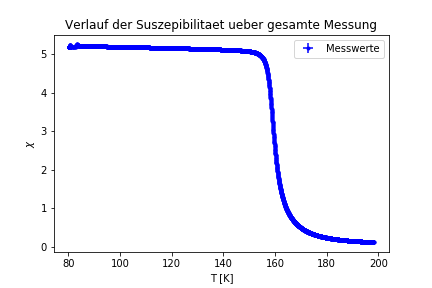
\includegraphics[scale=1]{Bilder/Haupt_Probe/Suszeptibilitaet_Verlauf.png}
\caption[test]{Verlauf der Suszeptibilität über die gesamte Messung.}
\label{fig:Suszeptibilitaet_Verlauf}
\end{figure}

Für die Messung der Probe wurde eine Phase von \SI{180}{\degree} verwendet, daher sind die Daten an der X-Achse gespiegelt. Zudem ist ein sehr großer Offset in den Daten, der noch zu bestimmen ist. \\
Für die Umrechnung der in der Messung aufgenommenen Spannung nach Korrektur des Offset in Suszeptibilität gilt folgender Zusammenhang:
\begin{equation*}
\chi = \dfrac{U}{C \cdot v \cdot V_{Probe} \cdot (1-n_M)}
\end{equation*}
Dabei sind
\begin{equation*}
C = 8034,7 \, \pm \, 34,7
\end{equation*}
die mit dem Supraleiter bestimmte Kalibrationskonstante, 
\begin{equation*}
V_{Probe} = \SI{22,90 \pm 0,05}{mm^3}
\end{equation*}
das Probenvolumen,
\begin{equation*}
n_M = 0,27
\end{equation*}
der Entmagnetisierungsfaktor und 
\begin{equation*}
v = \dfrac{\SI{10}{V}}{s}
\end{equation*}
der Verstärkungsfaktor, wobei $s$ die Sensitivität ist, die in diesem Versuch auf \SI{1}{mV} gestellt werden musste, da der Lockin-Verstärker ansonsten in einen Overload gelaufen wäre. Abbildung \ref{fig:Suszeptibilitaet_Verlauf} zeigt den Verlauf der Suszeptibilität der Probe über die gesamte Messung. 

\subsubsection{Curie-Weiss-Gesetz}
Für einen Temperaturbereich deutlich oberhalb der Grenztemperatur $T_C$ gilt der Zusammenhang:
\begin{equation*}
\chi ^{-1} = \dfrac{T - T_C}{C_{Curie}}
\end{equation*}
Dabei ist $C_{Curie}$ die materialabhängige Curie-Konstante. Daher ergibt sich bei Auftragung von $\chi ^{-1}$ gegen T ein linearer Zusammenhang. In Abbildung \ref{fig:Suszeptibilitaet_Verlauf} ist zu erkennen, dass die Grenztemperatur bei ca. \SI{160}{K} liegt, sodass der Bereich für diese Anpassung gewählt wird zu \SI{180}{K} - \SI{190}{K}. \\
Mit dieser Anpassung wird der Offset gewählt. Dazu wird die Anpassung für verschiedene Offsets in einem Bereich von \SI{0}{V} bis \SI{1,8}{V} in 10000 äquidistanten Schritten durchgeführt und derjenige Offset verwendet, der in der Anpassung das niedrigste $\chi ^2$/ndof ergeben hat. Dieses liegt mit 0.34 zu niedrig, es wurden also vermutlich die Fehler überschätzt.

\begin{figure}
\centering
\includegraphics[scale=1]{Bilder/Haupt_Probe/CurieWeiss.png}
\caption[test]{Lineare Anpassung bei Auftragung von $\chi ^{-1}$ gegen T in einem Bereich von \SI{180}{K} - \SI{190}{K}.}
\label{fig:CurieWeiss}
\end{figure}

Abbildung \ref{fig:CurieWeiss} zeigt die lineare Anpassung bei dem bestimmten Offset. Die Grenztemperatur berechnet sich aus den Anpassungsparametern zu:
\begin{equation}
T_C = -\dfrac{b}{a}
\label{eq:ProbeGrenztemperatur}
\end{equation}
Die Fehler auf die Parameter pflanzen sich fort zu:
\begin{equation}
\dfrac{\sigma _{T_C}}{T_C} = \sqrt{\left( \dfrac{\sigma _a}{a} \right)^2 + \left( \dfrac{\sigma _b}{b} \right)^2}
\label{eq:ProbeGrenztemperaturFehler}
\end{equation}
Der Wert für die Grenztemperatur ergibt sich zu (systematische Fehler werden später betrachtet):
\begin{equation*}
T_C^{(1)} = \SI{162,800 \pm 0,057}{K}
\end{equation*}

\subsubsection{Temperaturen nahe der Grenztemperatur}

\begin{figure}
\centering
\includegraphics[scale=1]{Bilder/Haupt_Probe/CurieWeiss_gamma.png}
\caption[test]{Lineare Anpassung bei Auftragung von $\chi ^{\frac{-1}{\gamma}}$ gegen T in einem Bereich von \SI{170}{K} - \SI{180}{K}.}
\label{fig:CurieWeiss_gamma}
\end{figure}

In einem Bereich nah an der Grenztemperatur wird der Zusammenhang besser beschrieben durch:
\begin{equation*}
\chi ^{-1} \propto (T - T_C)^\gamma
\end{equation*}
Wobei für den kritischen Exponenten des Phasenübergangs $\gamma \approx \dfrac{4}{3}$ gilt. \\
Es wird der Offset verwendet, der sich bei der ersten Anpassung als der beste herausgestellt hat. \\
Bei Auftragung von $\chi ^{\frac{-1}{\gamma}}$ gegen T ergibt sich erneut ein linearer Zusammenhang, an den ebenfalls eine Anpassung durchgeführt wird. Der Bereich für diese Anpassung wurde gewählt zu \SI{170}{K} - \SI{180}{K}. Diese Anpassung ist in Abbildung \ref{fig:CurieWeiss_gamma} dargestellt. Die Anpassung kann bei einem $\chi ^2$/ndof von 2.84 als gelungen betrachtet werden. Die Grenztemperatur und der Fehler bestimmen sich gemäß Gl. \ref{eq:ProbeGrenztemperatur} und Gl. \ref{eq:ProbeGrenztemperaturFehler} zu:
\begin{equation*}
T_C^{(2)} = \SI{156,862 \pm 0,061}{K}
\end{equation*}

\subsubsection{Temperaturgradient}

\begin{figure}
\centering
\includegraphics[scale=1]{Bilder/Haupt_Probe/Temperatur_Verlauf.png}
\caption[test]{Temperaturverlauf bei der Messung der Probe.}
\label{fig:TemperaturverlaufProbe}
\end{figure}

\begin{figure}
\centering
\includegraphics[scale=1]{Bilder/Haupt_Probe/Temperaturgradient_Verlauf.png}
\caption[test]{Verlauf des Temperaturgradienten bei der Messung der Probe.}
\label{fig:TemperaturgradientverlaufProbe}
\end{figure}

Bei der Messung wird in Intervallen \SI{200}{ms} u.a. die Temperatur gemessen. Damit ergibt sich der in Abbildung \ref{fig:TemperaturverlaufProbe} gezeigte Temperaturverlauf. \\
Den Temperaturgradienten erhält man nun aus der Ableitung des Temperaturverlaufs. Da die Datenpunkte deutlich schwanken, wird diese Ableitung bestimmt, indem immer an 20 Punkte eine lineare Regression durchgeführt wird. Der Mittelwert der Zeiten der 20 Temperaturpunkte und die Steigung ergeben dann Punktepaare des Temperaturgradienten. Der Verlauf des Temperaturgradienten ist in Abbildung \ref{fig:TemperaturgradientverlaufProbe} dargestellt. Daran ist deutlich zu sehen, dass der Temperaturgradient bei der Messung der Probe bis zu einer Temperatur von ca. \SI{180}{K} oberhalb der ursprünglich gesetzten Grenze von \SI{0,1}{K/s} liegt.

\subsubsection{Systematischer Fehler}
Die statistischen Fehler auf die aus den beiden Methoden bestimmten Grenztemperaturen sind sehr klein gegen die Differenz der beiden. Daher ist eine Betrachtung der Systematiken sehr wichtig. \\
Fehlerquelle, die als systematisch betrachtet werden kann, sind die Fehler auf die Werte, die zur Umrechnung von der Spannung auf die Suszeptibilität verwendet werden. Die Fehler pflanzen sich fort durch: 
\begin{equation*}
\dfrac{\sigma _{\chi}}{\chi} = \sqrt{\left( \dfrac{\sigma _C}{C} \right)^2 + \left( \dfrac{\sigma _v}{v} \right)^2 + \left( \dfrac{\sigma _V}{V} \right)^2 + \left( \dfrac{\sigma _{n_M}}{1 - n_M} \right)^2}
\end{equation*}
Dabei entstammt der Fehler auf die Kalibrationskonstante der Bestimmung derselben. Der Fehler auf das Probenvolumen bestimmt sich durch gaußsche Fehlerfortpflanzung aus den Ablesefehlern auf die mit einer Schieblehre gemessenen Dimensionen der Probe. Auf den Entmagnetisierungfaktor wird der Digitalisierungsfehler angenommen und auf den Verstärkungsfaktor ein Fehler von 5\% angenommen. Nun wird die Suszeptibilität um diesen Fehler in beide Richtungen verschoben und die Anpassungen erneut durchgeführt. Aus der Veränderung des Ergebnisses für die Grenztemperatur ergibt sich der systematische Fehler aus den Fehlern auf Kalibrationskonstante, Probenvolumen, Verstärkungsfaktor und Entmagnetisierungsfaktor, sodass sich insgesamt für die Grenztemperaturen die folgenden Werte ergeben:
\begin{equation*}
T_C^{(1)} = (162,800 \pm 0,057 \; (stat.) \; \; ^{+0,0000090}_{-0,0000086} \; (sys.)) \, \si{K}
\end{equation*}
\begin{equation*}
T_C^{(2)} = (156,8623 \pm 0,0615 \; (stat.) \; \; ^{+5,9370}_{-0,0030} \; (sys.)) \, \si{K}
\end{equation*}
Drei der vier Fehler (vier Fehler durch die Asymmetrie) sind eine Größenordnung oder mehr kleiner als die statistischen Fehler. Der vierte Fehler ist zwei Größenordnungen größer als der statistische Fehler und sorgt dafür, dass die beiden Werte für die Grenztemperatur innerhalb ihrer Fehler übereinstimmen. Woher der große Unterschied der systematischen Fehler kommt, ist unklar. \\
Dazu kommt noch ein Fehler durch den zu hohen Temperaturgradienten während der Messung. Den Betrag dieses Fehlers abzuschätzen ist schwierig. Da sich allerdings die Si-Diode, die zur Messung der Temperatur verwendet wird, unter dem Hartshorn-Spulensystem befindet, ist die gemessene Temperatur bei zu großem Temperaturgradient kleiner als die Temperatur der Probe. Dies liegt daran, dass der Probenstab nicht vollständig aus dem Dewar gezogen wird, sodass die Kühlung, die das Aufwärmen verlangsamt, die Diode und das Spulensystem von unten kühlt. Da der Temperaturgradient in dem Bereich, in dem die Anpassung für $T_C^{(1)}$ durchgeführt wurde, kleiner ist, als der Bereich, in dem die Anpassung für $T_C^{(2)}$ durchgeführt wurde, ist davon auszugehen, dass dieser Effekt die beiden Werte ''zusammenschieben''  würde.

\subsubsection{Zusammenfassung}

\begin{figure}
\centering
\includegraphics[scale=1]{Bilder/Haupt_Probe/Anteilbestimmung.png}
\caption[test]{Zusammensetzung der Probe in Abhängigkeit der Grenztemperatur\footnotemark.}
\label{fig:AnteilbestimmungProbe}
\end{figure}
\footnotetext{Quelle: Versuchsanleitung Seite 32.}

Die beiden Anpassungsbereiche haben Grenztemperaturen von $T_C^{(1)} = \SI{162,800 \pm 0,057}{K}$ und $T_C^{(2)} = \SI{156,862 \pm 0,061}{K}$ (mit statistischen Fehlern) ergeben. Die systematischen Fehler aus den Fehlern auf die Kalibrationskonstante, auf das Probenvolumen, auf den Verstärkungsfaktor und auf den Entmagnetisierungsfaktor wurden mit der Verschiebemethode bestimmt und sind asymmetrisch. Drei der vier systematischen Fehler sind deutlich kleiner als die statistischen, aber der vierte ist deutlich größer und sorgt alleine dafür, dass die Werte innerhalb ihrer Fehler übereinstimmen. Der Fehler durch einen zu großen Temperaturgradienten konnte nur qualitativ betrachtet werden, würde die Differenz der beiden Werte aber nochmal verringern. \\
Mit der Grenztemperatur kann nun anhand Abbildung \ref{fig:AnteilbestimmungProbe} die Zusammensetzung der Probe durch Ablesen bestimmt werden. Bei einer Grenztemperatur um \SI{160}{K} ergibt sich so ein Zn-Anteil von $x = 0.75$. Damit handelt es sich um eine GdAg$_{0.25}$Zn$_{0.75}$-Probe.


\section{Fazit}

\end{document}
